
\documentclass[a4paper,12pt,twoside]{ThesisStyle}


\usepackage{amsmath,amssymb}             % AMS Math
% \usepackage[french]{babel}
\usepackage[UKenglish]{babel}
\usepackage[utf8]{inputenc}
\usepackage[T1]{fontenc}
%\usepackage[left=1.5in,right=1.3in,top=1.1in,bottom=1.1in,includefoot,includehead,headheight=13.6pt]{geometry}
\usepackage[left=1.3in,right=1.0in,top=1.0in,bottom=1.0in,includefoot,includehead,headheight=15.0pt]{geometry}
\renewcommand{\baselinestretch}{1.05}
\usepackage{caption}
% for boxes and code snippet
\usepackage{fancybox}
\usepackage{listings}

% Table of contents for each chapter
\usepackage[nottoc, notlof, notlot]{tocbibind}
\usepackage{minitoc}
\setcounter{minitocdepth}{2}
\mtcindent=15pt
% Use \minitoc where to put a table of contents

\usepackage{aecompl}
\usepackage{xcolor}

% Glossary / list of abbreviations

\usepackage[intoc]{nomencl}
\renewcommand{\nomname}{List of Abbreviations}

\makenomenclature

% My pdf code

\usepackage{ifpdf}

\ifpdf
  \usepackage[pdftex]{graphicx}
  \DeclareGraphicsExtensions{.jpg}
  \usepackage[a4paper,pagebackref,hyperindex=true]{hyperref}
\else
  \usepackage{graphicx}
  \DeclareGraphicsExtensions{.ps,.eps}
  \usepackage[a4paper,dvipdfm,pagebackref,hyperindex=true]{hyperref}
\fi

\graphicspath{{.}{images/}}

% Links in pdf
\usepackage{color}
\definecolor{linkcol}{rgb}{0,0,0.4} 
\definecolor{citecol}{rgb}{0.5,0,0} 

% Change this to change the informations included in the pdf file

% See hyperref documentation for information on those parameters

\hypersetup
{
bookmarksopen=true,
pdftitle="Design and Use of Anatomical Atlases for Radiotherapy",
pdfauthor="Olivier COMMOWICK", 
pdfsubject="Creation of atlases and atlas based segmentation", %subject of the document
%pdftoolbar=false, % toolbar hidden
pdfmenubar=true, %menubar shown
pdfhighlight=/O, %effect of clicking on a link
colorlinks=true, %couleurs sur les liens hypertextes
pdfpagemode=None, %aucun mode de page
pdfpagelayout=SinglePage, %ouverture en simple page
pdffitwindow=true, %pages ouvertes entierement dans toute la fenetre
linkcolor=linkcol, %couleur des liens hypertextes internes
citecolor=citecol, %couleur des liens pour les citations
urlcolor=linkcol %couleur des liens pour les url
}

% definitions.
% -------------------

\setcounter{secnumdepth}{3}
\setcounter{tocdepth}{2}

% Some useful commands and shortcut for maths:  partial derivative and stuff

\newcommand{\pd}[2]{\frac{\partial #1}{\partial #2}}
\def\abs{\operatorname{abs}}
\def\argmax{\operatornamewithlimits{arg\,max}}
\def\argmin{\operatornamewithlimits{arg\,min}}
\def\diag{\operatorname{Diag}}
\newcommand{\eqRef}[1]{(\ref{#1})}

\usepackage{rotating}                    % Sideways of figures & tables
%\usepackage{bibunits}
%\usepackage[sectionbib]{chapterbib}          % Cross-reference package (Natural BiB)
%\usepackage{natbib}                  % Put References at the end of each chapter
                                         % Do not put 'sectionbib' option here.
                                         % Sectionbib option in 'natbib' will do.
\usepackage{fancyhdr}                    % Fancy Header and Footer

% \usepackage{txfonts}                     % Public Times New Roman text & math font
  
%%% Fancy Header %%%%%%%%%%%%%%%%%%%%%%%%%%%%%%%%%%%%%%%%%%%%%%%%%%%%%%%%%%%%%%%%%%
% Fancy Header Style Options

\pagestyle{fancy}                       % Sets fancy header and footer
\fancyfoot{}                            % Delete current footer settings

%\renewcommand{\chaptermark}[1]{         % Lower Case Chapter marker style
%  \markboth{\chaptername\ \thechapter.\ #1}}{}} %

%\renewcommand{\sectionmark}[1]{         % Lower case Section marker style
%  \markright{\thesection.\ #1}}         %

\fancyhead[LE,RO]{\bfseries\thepage}    % Page number (boldface) in left on even
% pages and right on odd pages
\fancyhead[RE]{\bfseries\nouppercase{\leftmark}}      % Chapter in the right on even pages
\fancyhead[LO]{\bfseries\nouppercase{\rightmark}}     % Section in the left on odd pages

\let\headruleORIG\headrule
\renewcommand{\headrule}{\color{black} \headruleORIG}
\renewcommand{\headrulewidth}{1.0pt}
\usepackage{colortbl}
\arrayrulecolor{black}

\fancypagestyle{plain}{
  \fancyhead{}
  \fancyfoot{}
  \renewcommand{\headrulewidth}{0pt}
}

\usepackage{algorithm}
\usepackage[noend]{algorithmic}
\usepackage[colorinlistoftodos]{todonotes}

%%% Clear Header %%%%%%%%%%%%%%%%%%%%%%%%%%%%%%%%%%%%%%%%%%%%%%%%%%%%%%%%%%%%%%%%%%
% Clear Header Style on the Last Empty Odd pages
\makeatletter

\def\cleardoublepage{\clearpage\if@twoside \ifodd\c@page\else%
  \hbox{}%
  \thispagestyle{empty}%              % Empty header styles
  \newpage%
  \if@twocolumn\hbox{}\newpage\fi\fi\fi}

\makeatother
 
%%%%%%%%%%%%%%%%%%%%%%%%%%%%%%%%%%%%%%%%%%%%%%%%%%%%%%%%%%%%%%%%%%%%%%%%%%%%%%% 
% Prints your review date and 'Draft Version' (From Josullvn, CS, CMU)
\newcommand{\reviewtimetoday}[2]{\special{!userdict begin
    /bop-hook{gsave 20 710 translate 45 rotate 0.8 setgray
      /Times-Roman findfont 12 scalefont setfont 0 0   moveto (#1) show
      0 -12 moveto (#2) show grestore}def end}}
% You can turn on or off this option.
% \reviewtimetoday{\today}{Draft Version}
%%%%%%%%%%%%%%%%%%%%%%%%%%%%%%%%%%%%%%%%%%%%%%%%%%%%%%%%%%%%%%%%%%%%%%%%%%%%%%% 

\newenvironment{maxime}[1]
{
\vspace*{0cm}
\hfill
\begin{minipage}{0.5\textwidth}%
%\rule[0.5ex]{\textwidth}{0.1mm}\\%
\hrulefill $\:$ {\bf #1}\\
%\vspace*{-0.25cm}
\it 
}%
{%

\hrulefill
\vspace*{0.5cm}%
\end{minipage}
}

\let\minitocORIG\minitoc
\renewcommand{\minitoc}{\minitocORIG \vspace{1.5em}}

\usepackage{multirow}


\newenvironment{bulletList}%
{ \begin{list}%
	{$\bullet$}%
	{\setlength{\labelwidth}{25pt}%
	 \setlength{\leftmargin}{30pt}%
	 \setlength{\itemsep}{\parsep}}}%
{ \end{list} }

\newtheorem{definition}{D�finition}
\renewcommand{\epsilon}{\varepsilon}

% centered page environment

\newenvironment{vcenterpage}
{\newpage\vspace*{\fill}\thispagestyle{empty}\renewcommand{\headrulewidth}{0pt}}
{\vspace*{\fill}}

\definecolor{mygreen}{rgb}{0,0.6,0}
\definecolor{mygray}{rgb}{0.5,0.5,0.5}
\definecolor{mymauve}{rgb}{0.58,0,0.82}

\lstset{ %
	backgroundcolor=\color{white},   % choose the background color; you must add \usepackage{color} or \usepackage{xcolor}; should come as last argument
	basicstyle=\footnotesize,        % the size of the fonts that are used for the code
	breakatwhitespace=false,         % sets if automatic breaks should only happen at whitespace
	breaklines=true,                 % sets automatic line breaking
	captionpos=b,                    % sets the caption-position to bottom
	commentstyle=\color{mygreen},    % comment style
	deletekeywords={...},            % if you want to delete keywords from the given language
	escapeinside={\%*}{*)},          % if you want to add LaTeX within your code
	extendedchars=true,              % lets you use non-ASCII characters; for 8-bits encodings only, does not work with UTF-8
	frame=single,	                   % adds a frame around the code
	keepspaces=true,                 % keeps spaces in text, useful for keeping indentation of code (possibly needs columns=flexible)
	keywordstyle=\color{blue},       % keyword style
	language=Octave,                 % the language of the code
	morekeywords={*,...},            % if you want to add more keywords to the set
	numbers=none,                    % where to put the line-numbers; possible values are (none, left, right)
	numbersep=5pt,                   % how far the line-numbers are from the code
	numberstyle=\tiny\color{mygray}, % the style that is used for the line-numbers
	rulecolor=\color{black},         % if not set, the frame-color may be changed on line-breaks within not-black text (e.g. comments (green here))
	showspaces=false,                % show spaces everywhere adding particular underscores; it overrides 'showstringspaces'
	showstringspaces=false,          % underline spaces within strings only
	showtabs=false,                  % show tabs within strings adding particular underscores
	stepnumber=2,                    % the step between two line-numbers. If it's 1, each line will be numbered
	stringstyle=\color{mymauve},     % string literal style
	tabsize=2,	                   % sets default tabsize to 2 spaces
	title=\lstname                   % show the filename of files included with \lstinputlisting; also try caption instead of title
}

\begin{document}

\begin{titlepage}
\begin{center}
\vspace*{2.0cm}
\noindent {\Large \textbf{Reactive Trajectory Planning in Structured    }} \\
\vspace*{0.2cm}
\noindent {\Large \textbf{Dynamic Urban Scenarios}} \\
\vspace*{0.2cm}
\noindent {\Large \textbf{with Static and Dynamic Obstacles}} \\
\vspace*{0.5cm}
\noindent \large {\bf Pradeep Korivi} \\
\vspace*{0.2cm}

\noindent \large {From the Faculty IV - Electrical Engineering and Computer Science} \\
\vspace*{0.2cm}
\noindent \large {Technische Universit{\"a}t Berlin} \\
\vspace*{0.2cm}
\noindent \large {Department of Telecommunication Systems -Communication and Operating Systems} \\
\vspace*{0.2cm}
\noindent \large {\bf Master of Science} \\
\vspace*{0.2cm}
\vspace{2cm}
{
\includegraphics[width=0.4\textwidth]{Images/university.png}}
\vspace*{2cm}
~\\
\begin{tabular}{ll}
	\noindent \large{ Guides :}	& \noindent \large{Prof. Dr.-Ing. Reinhardt Karnapke}\\
      \vspace*{0.1cm}
    \noindent \large{}	& \noindent \large{Prof. Dr. Habil. Odej Kao}\\
     
	
\end{tabular}

\vspace*{1.5cm}

\end{center}
\end{titlepage}
\sloppy

\titlepage

\chapter*{Abstract}
The goal of any motion planner is to achieve a driving trajectory that is collision free, smooth and responsive (reactive), at the same time being far-sighted to maintain consistency, deliberative and allow smooth transitions. Prior approaches solved this problem through different methods having various complexity levels. This thesis proposes an on road motion planner with combination of path-velocity combination along with a low computational overhead collision avoidance system. The reactive nature tunability of the proposed thesis is suitable for urban driving scenarios. 

\chapter*{Abstrakt}
To be translated
\begin{titlepage}
%\begin{center}
\vspace*{4.0cm}

\noindent\textbf{Eidesstattliche Erkl{\"a}rung}\newline
Ich best{\"a}tige, dass diese Masterarbeit meine eigene Arbeit ist und ich alle verwendeten
Quellen und Materialien dokumentiert habe. Diese Arbeit wurde zuvor keinem
anderen Pr{\"u}fungsausschuss vorgelegt und ist nicht ver{\"o}ffentlicht worden.

\vspace*{4.0cm}


\noindent \textbf{Statutory Declaration}\newline
I confirm that this Master's thesis is my own work and I have documented all sources
and material used. This thesis was not previously presented to another examination
board and has not been published.

\vspace*{1cm}
~\\
\begin{flushright}

\begin{tabular}{lc}
      \vspace*{0.1cm}
       &  ............................................ \\
      \vspace*{0.1cm}
					      & \noindent \large{Pradeep Korivi}\\
	  \vspace*{0.1cm}
					      & \noindent \large{Berlin, 11 May 2018 }
\end{tabular}

\end{flushright}

%\end{center}
\end{titlepage}
\sloppy

\titlepage


%\chapter*{Declaration}
%I declare that I have authored this thesis independently, that I have not used
%other  than  the  declared  sources/resources,  and  that  I  have  explicitly  marked
%all material which has been quoted either literally or by content from the used
%sources.\\
%Berlin, November 20, 2017
%Soumya Siladitya Mishra

\dominitoc

\pagenumbering{roman}

% \cleardoublepage

%\section*{Acknowledgments}
%
%Last thing to do :-)

\tableofcontents

\mainmatter

\chapter{Introduction}
\label{introduction}

Over the past years, autonomy has played a vital role in the development of automobiles. The vehicles have moved from being a pure mechanical wonder to a software and hardware combination. The developments are fuelled by development in low-cost sensor technology and government regulations to improve the safety of road transportation. At the same time, there is an increasing demand for fully autonomous vehicles with its potential in business services and safety of passengers.

The past decade has seen a great improvement in the development of technology for the autonomous vehicles bringing the science fiction of robots driving people a step closer. This technology has the potential for huge societal impacts by reducing the fatalities in car accidents to changing the ecosystem of transportation. It is reported by World Health Organization that there are more than 1.25 million deaths and between 20-50 million people suffering non-fatal injuries worldwide because of road accidents \cite{whoaccidents}. The accidents are because of many reasons such as road conditions, vehicle condition, driver alertness etc. The advancements in self-driving technology have a potential to reduce the risks by keeping track of road without distractions reducing human error and also react quicker in emergency situations.

Increase in the urban population in many cities around the world is leading to increased traffic congestion, this has effects on health and productivity of the people\cite{citycongestion}.Increase in congestion is a result of increase in car ownership, due to space constraints cities like Singapore are banning new car ownership \cite{singaporebanscars}. Autonomous cars have the potential to shape the future of transportation by promoting shared economy and reducing car ownership, thus contributing to the reduction in congestion of cities. 


\section{Motivation}

Autonomous vehicles are at the forefront of the research in current times, but to bring the technology closer to reality there needs to be further research, mainly to solve tougher problems of bringing autonomous vehicles to urban masses. Though robots can act deterministically, humans and environment are not deterministic with unexpected behaviours, thus making autonomous vehicles safe needs further research into understanding these interactions.

Full-scale autonomous vehicles are expensive, time taking, and safety critical to test in emergency scenarios, though simulators provide easy ways to evaluate the situations, physical aspect of the vehicle control is missing. Research into autonomous vehicles is an expensive endeavour with high costs on platforms, operational constraints and large teams involved. Model cars can break this barrier to bring the technology closer to a large number of researchers in the world thus being the enabler for greater innovation.

The challenges in autonomous vehicles can be subdivided into sensing/perception, navigation and control. The challenge under consideration in this thesis is the navigation/planning problem of driving the robot to the destination with available resources. The problem of navigation/trajectory planning challenge is special as the module is responsible for understanding the behaviour of the surrounding objects and adjust the ego vehicle's (vehicle in consideration for planning) behaviour accordingly following certain rules.

\section{Problem Statement}

The underlying problem of trajectory planning can be considered as a general robot path planning problem where the robot has to move on a planned route avoiding obstacles. There exist well-known methods within the domain of the robot path planning/ autonomous vehicles that can be adapted to achieve trajectory planning for model car. Model cars are limited to the available resources such as computational power, perception data, accuracy in measurements etc. Thus these approaches need to be tailor-made to suit the model car platforms.

Trajectory planning problem can be formulated as an optimal control problem to determine set of states $x(t)$ or controls $u(t)$ for a dynamic system (ego vehicle) over a time (planning horizon) to minimize a performance index. The index in context is minimizing the distance to goal following various constraints such no collision, maintaining the speed limit.

The challenge is to create trajectory planner considering limitations of these small platforms and achieving the behaviour of an autonomous car.

\section{Thesis Statement}

This thesis advocates that effective motion planning can be performed at a low computational cost by combining prediction and approximation techniques in trajectory creation and evaluation.

\section{Thesis Contributions}

The main contribution of this thesis is the introduction of a trajectory generation framework and algorithms for smaller model car platforms. The hierarchical framework employed divides the problem into four layers of planning named route planner, behavioural layer, trajectory planner and control node. The focus is the development of trajectory creation algorithm using samples of acceleration profiles and lateral shifts, an algorithm to pre-assign costs to samples such that planner evaluates the paths based on pre-costs and converges faster to the solution. The final contribution is collision detection algorithm that works in simple 2 steps for detecting collision with static and 3 steps for dynamic obstacles. 

\section{Thesis Structure}


The thesis is broadly organized as follows. The initial chapters present relevant research in this field, followed by a chapter outlining the target hardware and software platform setup, approach to motion planning. The approach is followed by implementation overview, evaluation and conclusion.

Firstly Chapter \ref{related_work} introduces the research direction in autonomous vehicles, followed by different planning approaches in on-road driving. Next, an overview of different trajectory representation and evaluation techniques is presented.

Chapter \ref{vehicle_info} provides a basic overview of the software and hardware architecture of the target platform.

Chapter \ref{planning_algo} provides a detailed illustration of the motion planning algorithms developed for this thesis followed by evaluation techniques to validate that the trajectories by checking for collision.

Chapter \ref{implementation} provides a basic overview of the implementation of the proposed planning algorithm, messages exchanged between layers.

Chapter \ref{evaluation} details on the different experiments performed to validate the planner followed by general criteria-based evaluation of the proposed planner.

Finally. Chapter \ref{conclusion} concludes regarding the work done in the thesis and throws some light at the future directions for the thesis.

%\include{Chapters/Concepts}
\chapter{Related Work}
\label{related_work}
Motion planning is a widely researched topic with roots in control, artificial intelligence, computational geometry and Robotics. The literature presented in \cite{book_robot_motion_planning}, \cite{book_lavelle_planning} review significant portion of standard planning techniques. Due to the complexity of the autonomous cars and the environments, general techniques from robotics cannot be applied. Planning for autonomous cars, in general, is subdivided into two categories namely planning in unstructured environments such as parking areas etc. and structured environments such as Road Networks where the traffic rules have to be followed. This chapter mainly focuses on the planning techniques in structured urban environments. The following subsections discuss regarding various approaches involved in planning, path representation techniques and finally regarding trajectory evaluation. 

\section{Planning Approaches}
\label{planning_aproaches}

Autonomous vehicles have been in research communities from 80's with projects such as PROMETHEUS \cite{prometheus}; the research was accelerated by competitions such as DARPA Grand Challenge in 2006 and DARPA Urban Challenge (DUC) in 2007 \cite{darpa_urban_challenge}. In DUC, six autonomous vehicles from different universities have completed the challenge and have used various techniques to accomplish the task. The methods developed during these events formed the basis for modern-day autonomous cars which perform with greater safety and comfort compared to the DUC participants. 

Approaches followed by different participants of DUC are described in \cite{darpa_urban_challenge}. All participants in the competition followed a similar procedure with differences in internal techniques to solve subproblems. Planning module of Boss, autonomous vehicle from Carnegie Melon University which won the DUC is described in general here. Its planning framework is mainly subdivided into three submodules 

\begin{itemize}
    \item Mission control: It is the higher level module which creates a global path, assigns lane to the vehicle to reach the checkpoints and detects blockades.
	\item Behavioral module: It is responsible for decisions such as precedence at intersections, lane change decision, speed planning, look ahead point assignment etc. 
	\item Motion planning module: It is responsible for generating local trajectories and converting them to steering and acceleration values. It initially creates a forward-looking path, and velocity planning is performed on top of that. 
\end{itemize}

After DUC, research efforts have been increased to develop state of the art solutions in perception, planning and control of autonomous vehicles. Motion planning plays a crucial role in the system with the aim of building trajectories that are collision free and also adhere to kinematic and dynamic constraints of vehicle, road boundaries and traffic rules \cite{motion_planning_techniques}. There have been numerous approaches to solving the problem of path planning, and some of them are discussed in this section. Potential fields is one of such algorithm, it models state space with attractive forces towards goal and repulsive forces near obstacles \cite{potential_field_3} \cite{potential_field_1} \cite{potential_field_2}. In this approach, a path is found by travelling along the steepest gradient of the potential field. However, there is a risk of paths getting trapped in local minima. The grid-based approach is another method used in Robotics, here environment is perceived as a set of grids and path is found travelling across these grids using algorithms like A*. The downside of these approaches is that the complexity increases exponentially with increase in grid resolution and grid size, there have been different variants of this approach as discussed in \cite{A_star} \cite{D_star_1} \cite{kolski_thesis}. A comprehensive study of various approaches in motion planning for autonomous vehicles is presented in \cite{motion_planning_techniques} \cite{survey_planning_techniques}.

Planning approaches that are widely used in autonomous driving are classified as shown in Figure \ref{related_work_classification}. The following subsections discuss research in each of the described categories. 

\begin{figure}
	\centering
	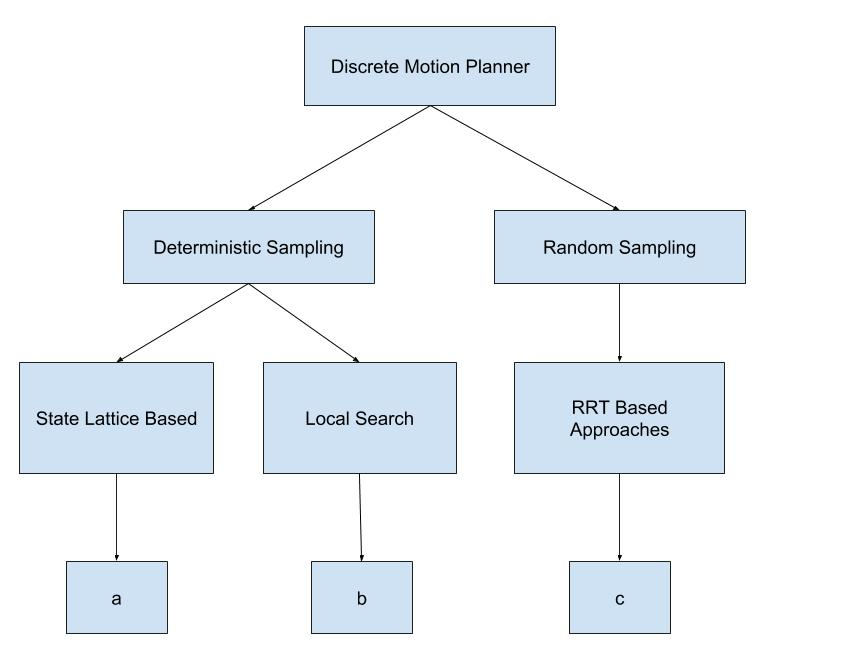
\includegraphics[width=0.8\textwidth]{Images/related_work/planning_division.jpg}
	\caption{General Overview of On-road planners. a - \cite{cmu_parallel_thesis}  \cite{diss_shui_phd_thesis} \cite{traj_planner_optimization} \cite{lattice_Gu_Tiyanu} \cite{unit_A_star} , b - \cite{kolski_thesis} \cite{real_time_traj_plan_article} \cite{darpa_urban_challenge}, c -\cite{rrt_star} \cite{rrt_urban_driv} \cite{mit_rrt1}
	}
	\label{related_work_classification}
\end{figure}

\subsection{Random Sampling Approaches}
\label{rw_incremental_search}
Rapidly-exploring Random Tree(RRT) technique was initially introduced by Steven M. LaValle in his work presented in \cite{Lavalle_rrt}. RRT builds a tree incrementally by sampling new states. In each iteration, a new sample $x$ is sampled and connected to the nearest neighbour $x_\textsubscript{neartest}$ in the tree if it is collision free. The tree starts at the start location and is built till the path to goal location is found. Probabilistic Roadmaps algorithm\cite{prm}(PRM) is another approach where uniform sampling is performed across the state space and are connected if a collision-free path exists. Then a graph search algorithm is employed to find a path from source to destination. Both of these approaches are probabilistic complete, i.e., as the number of samples increases the probability of finding a solution approaches one given problem is solvable.


Different variants of RRT's are widely accepted in robot motion planning because of its ability to explore higher dimensional problems at ease\cite{rrt_higher_dimension}. To improve the performance of RRT, bidirectional RRT with two trees(Bi-RRT) has been proposed. Though it enhances the performance, handling discontinuities between two trees are difficult\cite{birrt}. Environmentally guided RRT(EG-RRT) is another variant that incorporates information from scene analysis to guide samples and converge faster\cite{egrrt}. MIT has applied a closed loop prediction model into RRT(CL-RRT) in its autonomous vehicle at DUC \cite{mit_rrt}, a snippet of this planning approach is shown in Figure \ref{mit_rrt_fig}. In CL-RRT motion models are used to generate trajectories to sampled states and are evaluated for feasibility and performance. A variant named RRT* \cite{rrt_star} has been proposed which guarantee asymptotic optimality. In this approach, each state stores cost from the start and when a new sample is added, surrounding neighbours are tested if a better path can be found and the tree is rewired thus leading to an efficient path. There have been many techniques to reduce the number of sampled states in-order to save computational time, Informed-RRT \cite{informed_rrt} is one such approach which samples space according to the actual best path and states that are far away from the goal are not sampled.

\begin{figure}
	\centering
	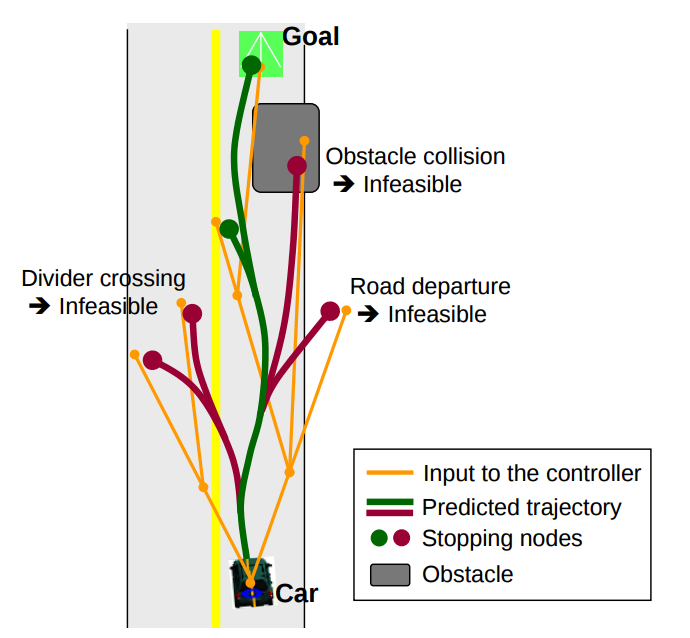
\includegraphics[width=0.6\textwidth]{Images/related_work/mit_urban_planning.png}
	\caption{MIT Darpa Urban Challenge - RRT based planning. In this approach, motion plans are propagated using vehicles dynamic model, and these paths are evaluated for feasibility}
	\label{mit_rrt_fig}
\end{figure} 

In real-world situations' environment is not entirely predictable and the computed path needs to be dynamically re-planned over the time. This replanning needs either a new plan to be generated quickly or rapid correction of old path. The approach Anytime-RRT \cite{anytimerrt} creates an initial path using RRT and optimises it on the go to create an optimal path, re-planning is triggered when the path is no longer valid. The method RRT$^x$ \cite{rrtx} updates the search space whenever obstacle changes are observed and repair the surrounding tree. 

Though RRTs are best-performing algorithms in planning, they exhibit certain deficiencies concerning motion planning for autonomous vehicles, especially in on-road driving conditions. RRT-based planners generate jerky and unnatural trajectories that contain many unnecessary turns\cite{improved_rrt}; these are suitable for open areas such as parking areas. Road parallel paths are preferred in structured environments.

\subsection{Lattice Planners}
\label{rw_lattice_planners}
The lattice planners use a discrete representation of the planning area with multiple states, each state is multidimensional with dimensions such as position, acceleration, velocity, time, curvature, heading etc. These states are connected, then the problem reduces to finding a path from the initial state to the final state in the lattice. This approach is well suited for non-holonomic robots and highly constrained areas such as road networks\cite{lattice_1}. Lattice planners are resolution complete, i.e., they can be automatically adjusted to change in resolution to explore state space consistently. The approach proposed in \cite{lattice_1} uses a multi-resolution state lattice with high resolution near start and goal locations and lower resolution in the middle to reduce computational complexity. Continuity of path and curvature are constraints in path planning, these are addressed in the research \cite{lattice_2} by defining a 4D configuration including 2D position, heading and steering. In \cite{cmu_parallel_thesis} the author added curvature to each state along with 2D position heading and curvature, paths between the vehicle and sampled sates are connected using third order spirals. A range of times and velocities are assigned to each vertex to enable spatiotemporal search. It uses constant acceleration profiles making it difficult for the vehicle to follow. Thus, due to a multitude of states involved, the number of trajectories created are in order of few hundred thousand. The number of trajectories to be evaluated increase exponentially if the state resolution is increased or new dimension is added. A graphical processing unit(GPU) is needed to run the evaluations in parallel to provide real-time response. 

To improve the performance of \cite{cmu_parallel_thesis}, the research published in \cite{traj_planner_optimization} utilizes quartic polynomials to ensure continuous curvature, connections are made from sampled endpoints and current state, Figure \ref{trajopt} shows further information about path and velocity representation. In this approach, speed profiles are generated inversely, and checks are included to ensure comfort, efficiency. To reduce the computational complexity the method proposed in \cite{traj_smoothing} uses a two-level planning approach which initially generates optimal collision-free reference path and then performs the search across this reference path to find an optimal trajectory. The reference path leads to a focused search and more human-like driving style. The research published in \cite{diss_shui_phd_thesis} further improves the trajectory smoothness ensuring a high level of trajectory diversity.

In summary, lattice planners create trajectories that are smooth, optimal and complying with dynamic and kinematic constraints of the vehicle. These approaches are well suited for structured and dynamic environments. They are also computationally expensive, and complexity increases exponentially with the addition of new state or increase in resolution.

\begin{figure}
	\centering
	\begin{subfigure}{.51\textwidth}
		\centering
		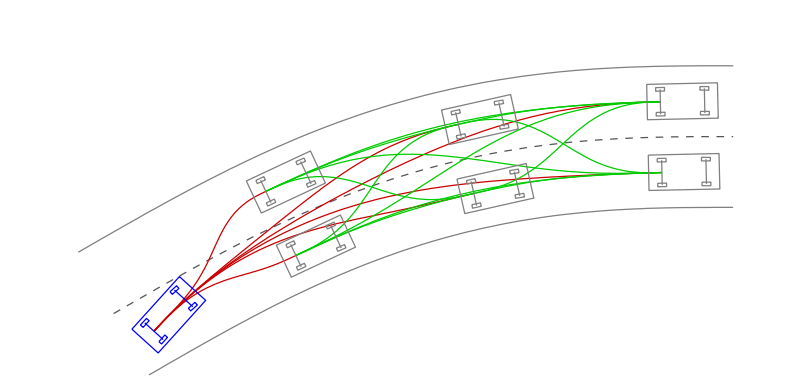
\includegraphics[width=1.0\linewidth]{Images/related_work/traj_optim_1.png}
		\caption{Path set. blue vehicle - current vehicle pose, and grey vehicles - sampled endpoints, red paths-quartic curvature polynomials and green paths - cubic ones}
		\label{trajoptsub1}
	\end{subfigure}\hspace{.01\textwidth}
	\begin{subfigure}{.47\textwidth}
		\centering
		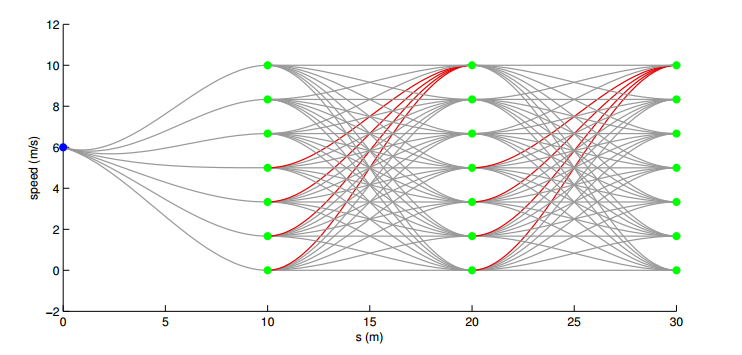
\includegraphics[width=1.0\linewidth]{Images/related_work/traj_optim_2.png}
		\caption{Speed set. The green points are sampled speeds at sampled longitudinal states, the red curves are beyond the acceleration limit, and the grey curves are valid ones}
		\label{trajoptsub2}
	\end{subfigure}
	\caption{Lattice Planner - Path velocity representation in \cite{traj_planner_optimization}}
	\label{trajopt}
\end{figure}

\subsection{Local Search}
\label{rw_local_search}

Local search is the most popular technique in autonomous driving, in this method instead of searching the complete graph a local state space is searched for a feasible solution as shown in \ref{cmubossduc}. The planners proposed in \cite{darpa_urban_challenge} \cite{juniorstanford} \cite{kolski_thesis} \cite{Broggi2012} \cite{real_time_traj_plan_article} \cite{urbansafetyeth} perform a variation of local search. In this approach a set of trajectories are forward projected based on vehicle dynamics, controls, to reach sampled states. The generated candidate trajectories are evaluated with a set of cost functions for collision checking and comfort to finalise the final trajectory. Paths with lateral shifts can be split into two categories, i.e., lateral shifts in action space(controls as a function of time and controls as a function of time and state) and state space(position, orientation, linear and angular velocities, curvature) of vehicle\cite{howard_phd}. Partial motion planning is another technique used to search locally reducing computational power significantly \cite{partialmotionplanning}. This technique has gained popularity due to ease in implementation and ability to perform rich sampling in short horizon for solving motion planning problem. In summary, local search algorithms can create short-term trajectories at a low computational cost with limitations in the manoeuvres robot can perform, these are especially suitable for low-speed and on-road driving.

\begin{figure}
	\centering
	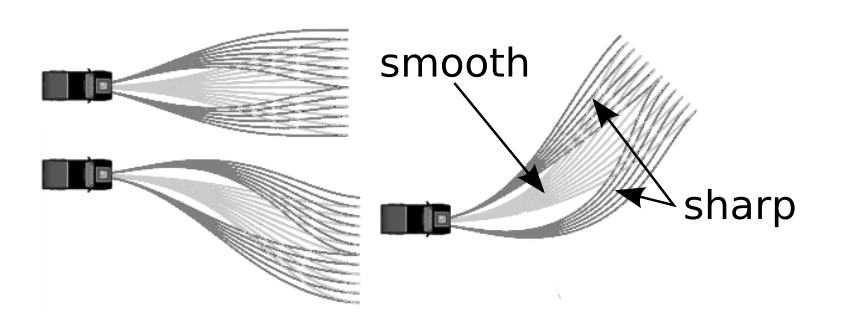
\includegraphics[width=0.6\textwidth]{Images/related_work/trajectorysetbossduc.png}
	\caption{CMU Darpa Urban Challenge - Local Search Forward projected trajectories}
	\label{cmubossduc}
\end{figure} 

\section{Trajectory Representation}
\label{trajrep}
Trajectory or path representation is another crucial factor in quantifying the trajectories; there are different methods such as arcs, second to fifth order polynomials, Cubic to Quintic Bezier curves, Dubian Paths, Reeds-Shepp curves, Akima splines, splines etc. Each of these curves has different advantages, disadvantages and suitable in different environments as discussed in \cite{motion_planning_techniques}. Splines and polynomials are used for creating road parallel trajectories, fifth order polynomials produce jerk minimising trajectories\cite{werling_frenet}, and other formats of trajectory representation mentioned earlier are employed by different planners discussed in previous sections. Reeds-shepp curves, a version of Dubian curves allow forward and backward driving \cite{reedsshepp} thus making them suitable for complicated manoeuvres in parking lots, obstacle course etc.


\section{Trajectory Evaluation}
\label{traj_eval}
Trajectory created by different methods mentioned in previous sections must be validated against various constraints to check feasibility, comfort, optimality and collision. The approach proposed in \cite{traj_planner_optimization} combines costs from different cost functions to check each trajectory for path length, curvature, the rate of change of curvature, lateral offset to the closest centre line, transformed distance to static obstacles, duration of the plan, speed, acceleration, jerk, centripetal acceleration, distance to dynamic obstacles to rank the trajectories. All the planners' test for some or all of the parameters mentioned using cost functions; some weigh each cost differently based on optimising factor, \cite{unit_A_star} penalise breaking to prefer long-range trajectories, \cite{cmu_parallel_thesis} penalises shorter horizons to ensure minimum horizon. Primary criteria for trajectory evaluation is collision checking to ensure safe motion and comfort.

Simulation-based techniques are widely used in collision checking where the vehicle is simulated in time to check for collision with other obstacles.

In \cite{kolski_thesis}, for collision checking in static environments, a map is represented as grid cells and based on obstacles and traversable areas the cells are assigned cost, and the trajectories that pass through these cells are added with corresponding costs as shown in Figure \ref{kolski1}. Finally, the trajectory with the lowest cost is selected. In dynamic environments' vehicle shape is forwarded and checked for collision with static obstacles as represented in Figure \ref{kolski2}.
\begin{figure}
	\centering
	\begin{subfigure}{.49\textwidth}
		\centering
		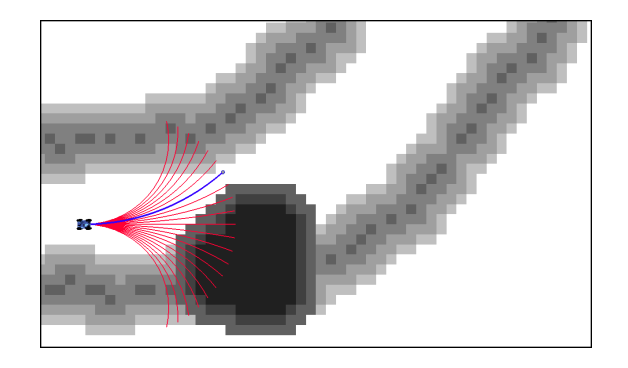
\includegraphics[width=1.0\linewidth]{Images/related_work/kolskistaticobst.png}
		\caption{Static Environments - Map is represented by a set of grid cells; the cells are assigned cost based on the presence of obstacle and closeness to obstacles. Cost of the path is computed based on the cost of the cells it traverses through, darker the cell higher the cost.}
		\label{kolski1}
	\end{subfigure}\hspace{.01\textwidth}
	\begin{subfigure}{.49\textwidth}
		\centering
		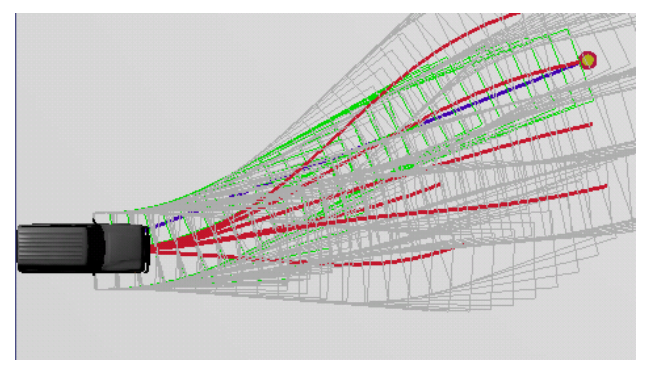
\includegraphics[width=1.0\linewidth]{Images/related_work/dynamiccollsionkolski.png}
		\caption{Dynamic Environments - The vehicle shape is forward projected for each path, and the collision checking is performed at each step. If at any point the shape of the ego vehicle collides with an obstacle, the path is marked invalid.}
		\label{kolski2}
	\end{subfigure}
	\caption{Collision Checking for Static Obstacles \cite{kolski_thesis}}
	\label{kolskicollison}
\end{figure}

For collision checking with dynamic obstacles, \cite{kolski_thesis} uses a hierarchical approach. In this method initially given vehicle trajectory and obstacle trajectory bounding boxes are constructed and checked for collision, if they intersect then in incremental time steps a pessimistic approximation of circles is used to check for collision, if they also collide then actual model of the car is used to check for collision as represented in Figure \ref{kolskidynamicobst}.

\begin{figure}
	\centering
	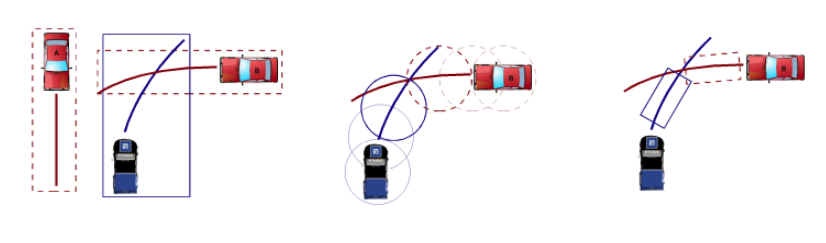
\includegraphics[width=1.0\textwidth]{Images/related_work/kolskidynamicobstacles.png}
	\caption{Collison checking for Dynamic Obstacles \cite{kolski_thesis} a) Initially bounding boxes along length of trajectory are drawn to determine if the trajectories collide, if they collide b) circle approximating the shape of the ego is forward projected and checked for collision, if this is also colliding then c) shape of the ego is forward projected and checked for collision.}
	\label{kolskidynamicobst}
\end{figure} 

In \cite{cmu_parallel_thesis}, for collision checking with respect to static obstacles, each (x,y) point in world is assigned a cost based on proximity to static obstacles, a path that intersects with obstacles has lethal cost, paths that have proximity to these obstacles have high costs and paths that are away from obstacles are assigned zero cost. A Potential function is created based on the position of obstacles to that computes the cost of the path. Similarly, for dynamic obstacles, a potential function is created by adding t dimension to create cost function in (x,y,t). Static and dynamic obstacles are dilated accordingly to remove errors in perception and ensure safety.


In \cite{rrt_star} collision checking is performed by forward projecting the vehicle shape represented as rectangle and collision checking with lines joining the initial and final state of obstacles and border lines. The planner proposed in \cite{volvo_reactive_traj} presents a reactive approach, in this distance to the dynamic obstacles ahead, is used as a parameter to stop the vehicle.

The approaches proposed for collision checking rely on predicting future trajectory by assumptions that obstacles will continue with constant velocity, acceleration, current orientation, in the same lane etc., these assumptions are not accurate and may lead to inefficiencies due to ignoring traffic context, interactions between vehicles etc. \cite{motion_planning_techniques}. There are also uncertainties in data predicted by the perception module, and they must be considered while collision checking.

In summary, collision checking is an important and also a complex task which involves different types of checks, assumptions, and approximations to create trajectories that are safe.


%Look if the sampling based, RRT based, lattice based etc etc should be combined together?
%write about MDP, POMDP etc 
\chapter{Target Platform}
\label{vehicle_info}

\begin{figure}[H]
	\centering
	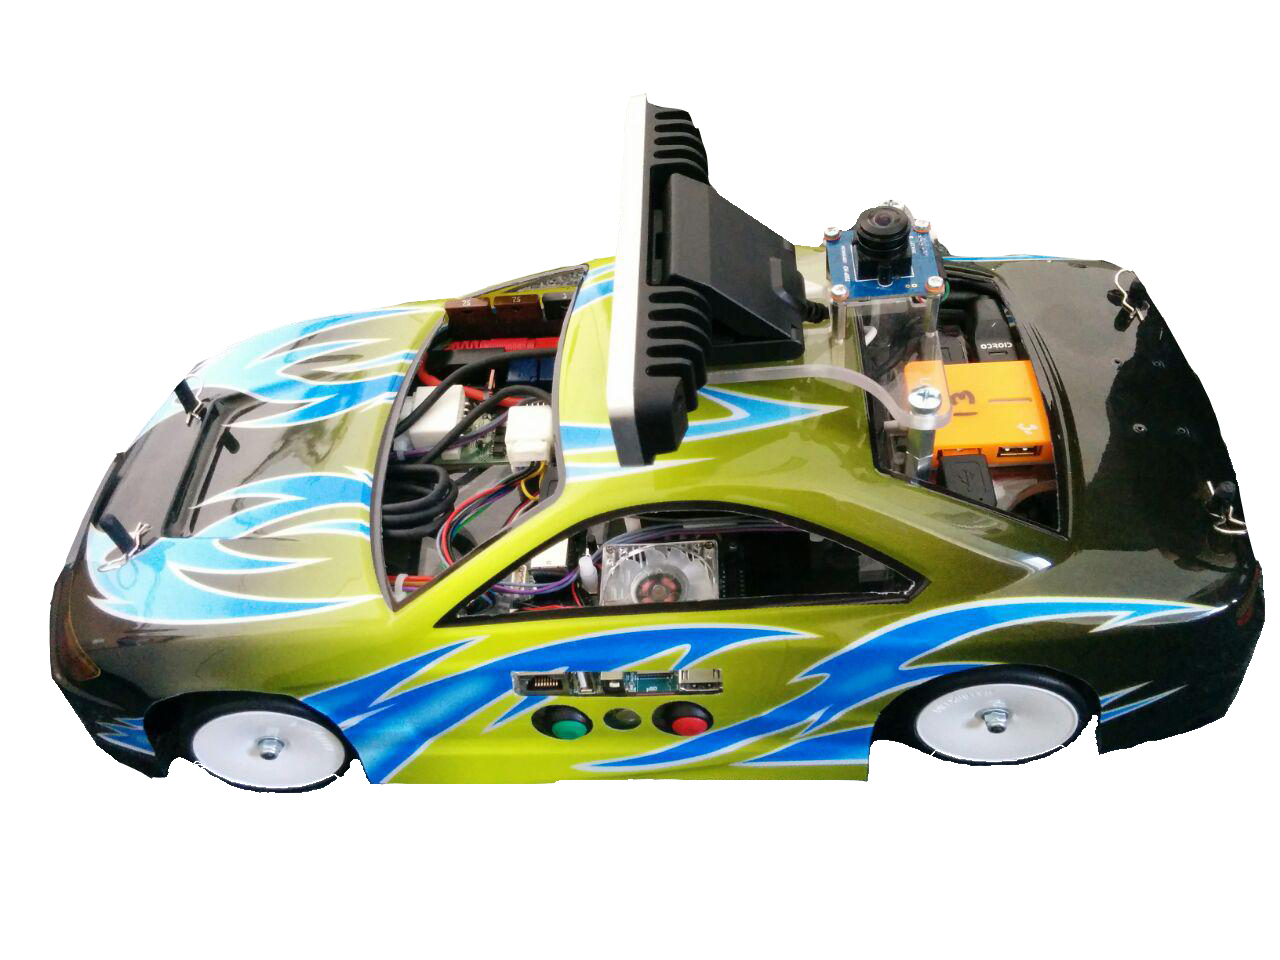
\includegraphics[width=0.6\textwidth]{Images/platform/car.jpg}
	\caption{Model car external view}
	\label{model_car}
\end{figure}

\section{Hardware Components}
The target platform for validating the planner is a 1:10 scale model car (AutoNOMOS Mini V3) as shown in Figure \ref{model_car}, it is developed as an education and research platform. The car is a modified RC platform, different hardware components used are described in Figure \ref{internalcar}. The main components are a Brushless DC-Servomotor (FAULHABER 2232) to drive and measure speed, a servo motor (HS-645MG) to control the Ackerman steering, IMU (MPU6050) to measure the orientation of the car. The three modules mentioned are controlled with an Arduino Nano which communicates the data to the main CPU (Odroid XU4 - Embedded Computer). Other important components are a depth camera (realsense sr300) for forward vision and perceiving the shape of obstacles ahead, 2D-Lidar (RPLidar), WiFi Dongle, Fisheye Camera for localizing car based on markers on the roof. The Figure \ref{moduleconnections} presents connections across different modules present in the car.
\begin{figure}
	\centering
	\includegraphics[width=0.8\textwidth]{Images/platform/car_internals.png}
	\caption{Internal components of Model Car}
	\label{internalcar}
\end{figure}

\begin{figure}
	\centering
	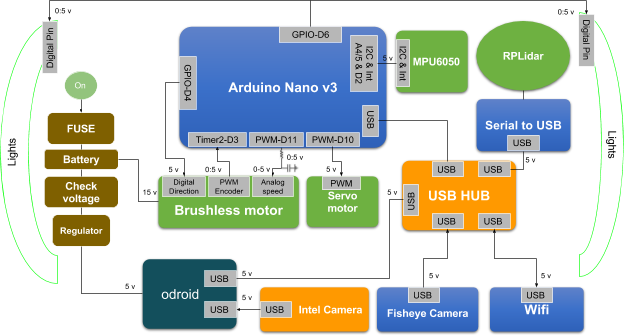
\includegraphics[width=0.8\textwidth]{Images/platform/hardware_Connections.png}
	\caption{Module Connections}
	\label{moduleconnections}
\end{figure}

\section{Software Components}
The CPU onboard runs Robot Operating System (ROS) on top of Ubuntu. ROS is a widely known framework for robotics applications due to its modularity and distributed nature. Modularity allows the application designer to choose which modules to be developed and which modules to be used directly. There are thousands of packages available open-source developed by the community which help to realize a project in a short time. The distributed nature of ROS allows to distribute modules across different platforms based on hardware requirements and communicate easily across them.

The model car implements core components for motor control, reading data from sensors, Odometry, Camera interfaces etc. There are community developed packages for visual GPS to track markers on the roof and localize car, line detection, traffic sign detection etc.

In summary, the model car features all the components to drive the car autonomously, but there are limitations on the accuracy of measurements, control and computational resources on board. 

%\section{Sensors}
%\section{Architecture \& Computational Power}
%\section{Vehicle Control}
%\section{Localisation}

\chapter{Planning Algorithm}
\label{planning_algo}
\section{Introduction}

The goal of the path planner is to navigate the robot from the start state to destination by blending in the traffic. Path planning module is dependent on various modules to receive the data regarding the perceived environment and invoke a set of modules to move the ego vehicle safely. It has to drive the ego vehicle forward considering the traffic rules, obstacles, kinematic and dynamic constraints of the robot and not compromising on the safety and comfort of the passengers inside. This chapter aims to describe path planning techniques developed in this thesis to drive the ego vehicle safely to the destination.

This section is organised to provide an overview of different modules needed for path planning and methods used in each module to achieve the goal. Path planning starts from the initial understanding of where the ego vehicle is and where to go, subsection \ref{localization} describes the localisation of ego vehicle to provide this data, subsection \ref{route_planner} provides the information on how a global path to the destination is calculated. An autonomous vehicle should have an understanding of surroundings concerning where other vehicles are, where pedestrians are, traffic signal information etc. Prediction module described in \ref{prediction} details further on how the ego vehicle perceives the environment. The next subsection \ref{motion_planner} describes in-depth details on the short-term planning algorithm aka trajectory planner. The final module in the discussion is control unit, described in subsection \ref{traj_follower}. It is responsible for translating the path in space-time into steering and acceleration values to drive the ego vehicle.

Figure \ref{path_planner} represents the general architecture of the planning module. It details on the flow of information, dependencies, relative execution frequency. The components in dark blue are the primary focus of this thesis, parts in light blue are adopted from other works and modules in sky blue are preexisting or simulated. 
\begin{figure}[h]
    \centering
    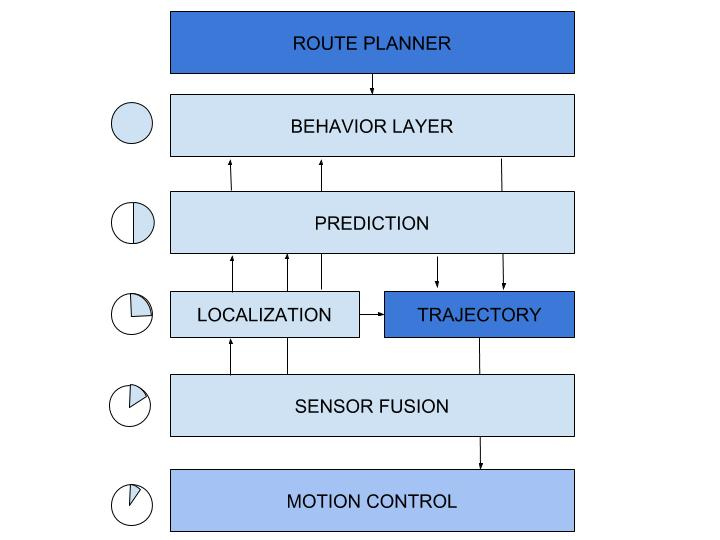
\includegraphics[width=0.8\textwidth]{Images/path_planner.jpg}
    \caption{Path Planning Module}
    \label{path_planner}
\end{figure}

\section{Localization} \label{localization}

Localization module is responsible for providing the current state of the vehicle concerning the position, orientation, speed(linear and angular) and acceleration. The localisation module implemented on the modelcar has two sub-components, Vehicle Odometry and a Visual GPS. Odometry is calculated with dead reckoning \cite{dead_reckoning} with speed information from motor and Yaw information from Inertial Measurement Unit (IMU). The localisation module combines odometry with the data received from a visual GPS node (tracks markers on the roof) to correctly estimate the state of the ego vehicle. 

\section{Prediction} \label{prediction}

Prediction and Sensor fusion modules receive the data from various sensors such as Cameras, LIDAR, etc. and fuse them together to create an environment model, classifying objects into different categories and predict the state of obstacles in the surroundings. Due to time constraints, this thesis simulates a prediction module to provide motion planner with obstacle information in different traffic scenarios.

\section{Route Planner} \label{route_planner}
Route Planner is responsible for finding a global route between the current vehicle state and the goal state based on the static characteristics of the environment/map such as lane information, speed limits etc. Route planner obtains this information generally from the maps or other formats to represent the road network. In this thesis a simple model called " Road Navigation Definition File (RNDF)"  \cite{rndf_darpa} \cite{rndf_fu} is used to represent the route network. Next subsections details further about RNDF and global reference route calculation.

\subsection{RNDF}

This section details about the RNDF file \cite{rndf_darpa} which defines the road network(set of roads/ areas connected) over which the vehicle can traverse. DARPA developed this representation of road for its Autonomous Vehicles Urban Grand Challenge. RNDF representation first divides the traversable areas into two parts, segments and free zones and provides connections across these areas. Free zones represent areas such as parking lots and road segments represent driving lanes. Each segment has multiple lanes; each lane has waypoints along the driving direction. More significant information about waypoints such as whether it is a stop sign, speed limit, start/end, intersection etc. can be added. Each segment/zone is connected to one another using exits, they represent the connections between one segment waypoints at start/end to another. Figures \ref{rndf_segment} \ref{rndf_exits} \ref{zone_segment} \cite{rndf_darpa} represent different portions of the route representation and Figure \ref{path_Segmentation} details regarding one of the route network of map used in Lab experiments. 


%\begin{figure}
%    \centering
%    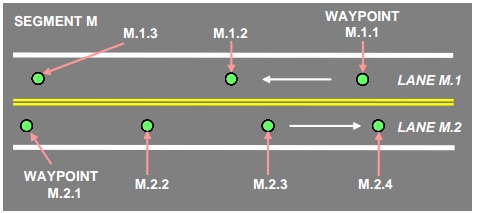
\includegraphics[width=0.6\textwidth]{Images/rndf_segment.png}
%    \caption{Segment representation in RNDF - Segement M has two lanes M1, M2 and each lane has way points 1-N}
%    \label{rndf_segment}
%\end{figure}

%\begin{figure}
%    \centering
%    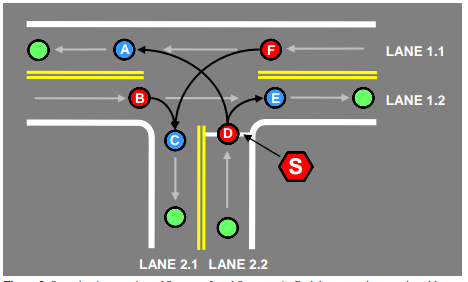
\includegraphics[width=0.5\textwidth]{Images/rndf_exits.png}
%    \caption{Exit representation in RNDF - Connections between two segments in a T-Junction}
%    \label{rndf_exits}
%\end{figure}


\begin{figure}
	\centering
	\begin{subfigure}{.55\textwidth}
	    \centering
		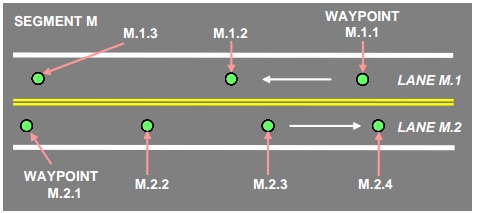
\includegraphics[width=1.0\textwidth]{Images/rndf_segment.png}
		\caption{Segment representation in RNDF - Segement M has two lanes M1, M2 and each lane has way points 1-N}
		\label{rndf_segment}
	\end{subfigure}\hspace{.01\textwidth}
	\begin{subfigure}{.43\textwidth}
		\centering
		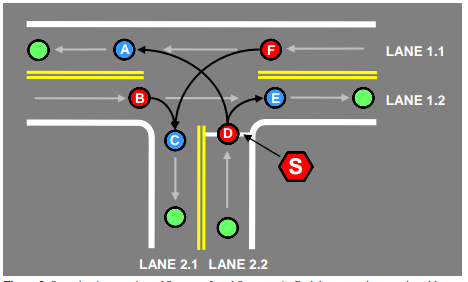
\includegraphics[width=1.0\textwidth]{Images/rndf_exits.png}
		\caption{Exit representation in RNDF - Connections between two segments in a T-Junction}
		\label{rndf_exits}
	\end{subfigure}
	\caption{Road representation in RNDF \cite{rndf_darpa}}
	\label{rndf_seg_exit}
\end{figure}

\begin{figure}
    \centering
    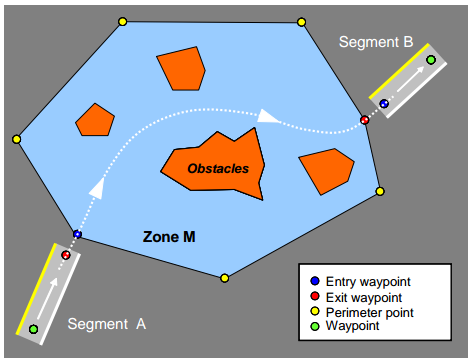
\includegraphics[width=0.5\textwidth]{Images/zone_segment.png}
    \caption{Connection between Segments and Zones (free paths) in RNDF \cite{rndf_darpa}}
    \label{zone_segment}
\end{figure}


%\begin{figure}
%    \centering
%    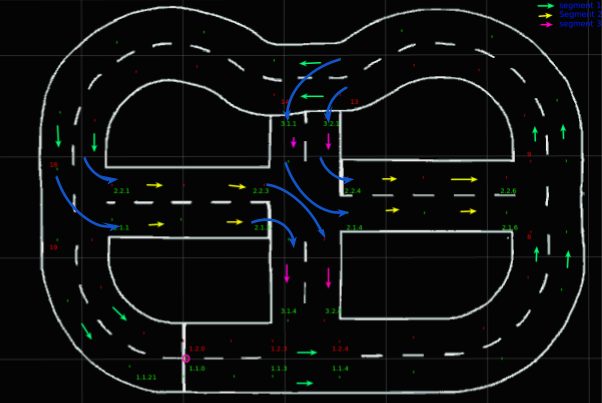
\includegraphics[width=0.8\textwidth]{Images/map_rndf.png}
%    \caption{Road network for the map used to test model Car}
%    \label{map_rndf}
%\end{figure}


\subsection{Path Representation and calculation}

The data in RNDF is represented in the form of a graph with connections across way-points as edges and way-points as vertices. The global path from source to destination is the shortest path between the waypoint closest to the ego vehicle's current position and the waypoint closest to the destination. The shortest path found is divided into sub-paths based on the segment to which the waypoints belong. Once the ego vehicle is at the end of one sub-path it receives a notification from the trajectory planner that a goal is reached, then the route planner transmits the next subpath to the trajectory planner, this process is repeated till destination is reached. Figure \ref{path_Segmentation} details further about the division of shortest path across different segments. This method also reduces the memory needed in modelling the road in trajectory planning stage.

\begin{figure}
    \centering
    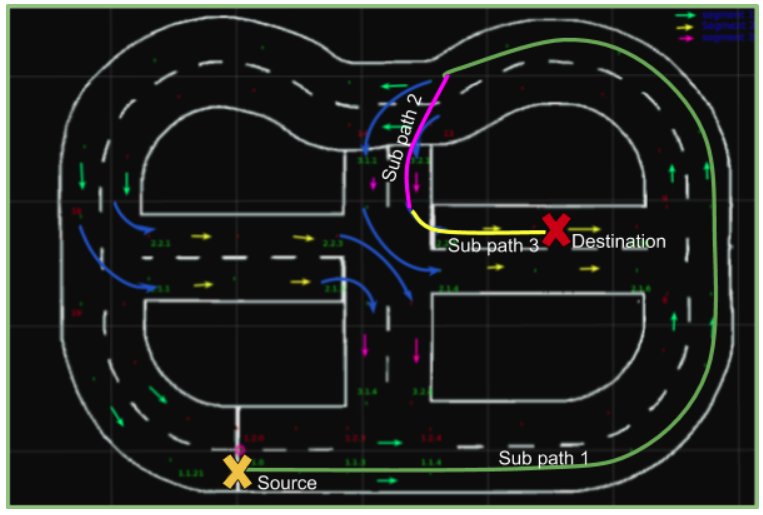
\includegraphics[width=0.8\textwidth]{Images/path_Segmentation.png}
    \caption{Division of shortest path in road network into Sub paths across different segments}
    \label{path_Segmentation}
\end{figure}

\subsection{Behavioural Layer}
Behavioural layer plays an essential role in path planning; it is responsible for understanding the scenario and making decisions according to various traffic rules, constraints and choices that make driving efficient. For example, it decides on target lane and speed based on information such as emptiness of road, other cars in the lane, next needed exit and turn, speed limit etc. The behavioural layer is a vast research topic in itself and not in the scope of this thesis. Currently, a simple simulated approach is implemented where the user can provide inputs to decide behaviour using mouse clicks for lane change and speed information from the map.

\section{Motion Planner} \label{motion_planner}
Motion Planning/Trajectory planning creates short-term space-time trajectories that drive the robot safely adhering to global path discussed in \ref{route_planner}. This section is organised into multiple subsections which describe each of the subproblems in creating local trajectories. The subsection \ref{timing_constraints} provides an overview of the timing Horizon and constraints in dynamic environments for different modules in planning. The next subsection \ref{frenet_frame} details regarding path modelling and how this will improve the efficiency of planning along with its constraints. It also discusses on approximation method used to convert coordinates from Cartesian to Frenet frame and vice versa. The core of this section is the creation of trajectories which is discussed in detail in subsection \ref{traj_creation}. The next subsections \ref{osbtacle_check_satic} and \ref{obstacle_check_dynamic} explain further on how the created trajectories are evaluated for collision with static and dynamic obstacles. Next subsection \ref{traj_Selection} details on the selection of final trajectory from the set of evaluated trajectories for trajectory following.

\subsection{Temporal Horizon} \label{timing_constraints}
Time is an essential aspect of planning in dynamic environments, and there are several timing variables associated with planning. This section is mainly adopted from the doctoral thesis "Autonomous vehicle navigation in dynamic urban environments for increased traffic safety" \cite{eth_timing_constraints}. These timing parameters define how far into the future different sub-modules of planning will be valid. 

The first timing variable in motion planning is timing horizon $ T_m $. It is the measure of how far into the future trajectory of the ego vehicle is planned. Second is the prediction horizon $ T_p $; it is the measure of how far into the future the motion of dynamic obstacles around the ego vehicle can be predicted. The fundamental requirement of planning to be valid is that $ T_m  \le  T_p $ such that planning is done only so far into the future as the environment is predictable. 

Third is $ T_d $, which indicates the computation time of the motion plan. Assuming planning is done in cycles, the plan created in the previous cycle is executed in the current cycle, thus $ T_d  \le  T_m $. If this condition fails, then the planner will run out of path for the next cycle. In general $ T_d \ll T_m $. The fourth timing variable $ T_s $ is the perception update cycle time, i.e., perception module updates the state of surrounding dynamic obstacles every $ T_s $ seconds. In general world, the predicted trajectories for duration $ T_p $ will not hold true, as the behaviour of these vehicles is not controlled by the ego vehicle. Thus the constraint $ T_s  \le T_p $ should be valid. This creates an uncertainty in modelling of the environment. Thus the execution duration of current plan $ T_e $ beyond $ T_s $ is not sensible; this is because obstacle trajectories may have changed in $ T_s $ and executing the old trajectory may lead to collisions invalidating the trajectory created for $ T_m $. 

The next timing constraint in consideration is $ T_e $, control execution time of the current plan. $ T_e $ should not exceed the perception update time $ T_s $. This restriction also imposes additional constraint on $ T_d $ (motion plan computation time), $ T_d \le T_e $. 

In summary, timing constraints described above identify the relation between different modules such as motion planning, motion prediction and execution. It is also important to predict farther into future than $T_s$ or $T_e$ for completeness of motion planner concerning goal objective. In general, a farsighted uncertain motion plan potentially directing the vehicle towards the goal is better, but this plan needs to be re-evaluated and re-executed in short intervals for correctness. 

In general behaviour of obstacles and participants can be predicted for up-to 5s probabilistically. Thus the temporal $ T_m $ \& prediction $ T_p $ horizon are chosen to be 5s. The planner has an execution time $ T_d $ far less than recommended 100ms on a low power computational hardware which allows a high update rate allowing lower values for $ T_e $. As obstacle detection is simulated, a pessimistic value of 250ms for $ T_s $ is chosen, and the planner is capable of handling higher update rate also. 

\subsection{Path Modelling} \label{frenet_frame}

 The planned global path is in the Cartesian coordinate system. One of the problems with the Cartesian coordinate system is that the due to variation in curvature of the road, local planning becomes complex. To address this issue planning in curvilinear system or Frenet Frame or  lane adoptive (SL) coordinate system has been adopted by researchers, \cite{traj_planner_optimization} \cite{spatio_temporal_state_lattice} \cite{diss_shui_phd_thesis} \cite{real_time_traj_plan_article} \cite{volvo_reactive_traj} \cite{curvilinear_System_Automated_Drv} are some of the research works in which Frenet frame is adopted. In this method centre of the lane/road or preplanned global path is used as reference longitudinal coordinate (S) and perpendicular distance with respect to the lane centre is considered as lateral coordinate (L/D) as represented in Figure \ref{sl_over_xy} \cite{diss_shui_phd_thesis}.  Thus once converted, (S, L) coordinate system essentially is a straight road.
 
 \begin{figure}
    \centering
    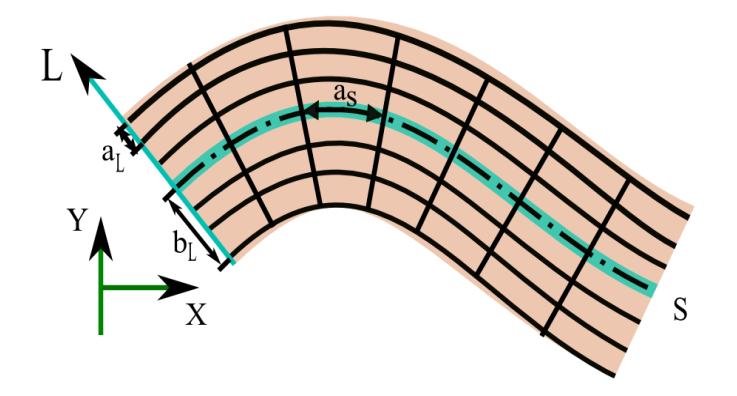
\includegraphics[width=0.8\textwidth]{Images/sl_over_xy.png}
    \caption{SL coordinate system laid over XY coordinate system - \cite{diss_shui_phd_thesis}}
    \label{sl_over_xy}
\end{figure}
 
 Conversion from Frenet frame to Cartesian and vice versa is a widely researched topic and many techniques exist which offer different levels of complexity and accuracy. In this thesis, an approximation method is used to convert between these two coordinate systems similar to \cite{volvo_reactive_traj}. This method is computationally inexpensive and provides a required level of accuracy for the model car. To convert an XY coordinate to SL coordinate, (x,y) is projected onto the current path represented by straight lines joining waypoints as in figure \ref{xy_sl_conversion}, cumulative distance till this point gives the S coordinate, and the perpendicular distance between the projected point and the current point provides the L coordinate. A similar process is used to convert S,L coordinate to x,y coordinate. S is used to find a point on a segment represented by waypoints, a point at a perpendicular distance L gives the x,y coordinate. We assume that the path between two waypoints is linear which reduces the computational complexity in approximation. This approximation, however, approaches zero error when the spacing between two waypoints approaches zero. Adding dense waypoints in the curves significantly reduces the approximation error. There are different methods discussed in \cite{lengthparameterized}, \cite{Wangrobustand} which provide better accuracy in calculating the paths. 

As observed in Figure \ref{sl_over_xy}, in SL coordinate system the size of the unit distance is not constant, it stretches in the convex side of the road and gets compressed in the concave side of the reference line. This is especially an issue in curves with a lower radius of curvature, as it affects velocity planning thus leading to discomfort in some cases. There is extensive research on the topic of velocity and path smoothening which counter these effects. 

In summary, the curvilinear coordinate system makes planning easier but needs extra computation in the conversion from one format to other. It also introduces some errors and inefficiencies in planning if the complete planning is done in SL coordinate system and these need to be addressed. 
 
 \begin{figure}
    \centering
    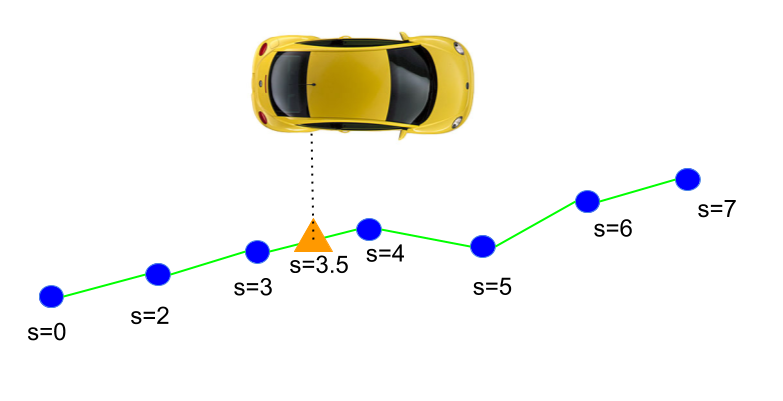
\includegraphics[width=0.8\textwidth]{Images/xy_sl_conversion.png}
    \caption{Showing projection of the current position of the car shown by green triangle to s coordinate system. Each circle represents a node, and the lines between them are links. \cite{volvo_reactive_traj}}
    \label{xy_sl_conversion}
\end{figure}

\subsection{ Trajectory Creation} \label{traj_creation}

The core of this thesis is the trajectory planner that drives the robot from source to destination. By understanding the behaviour of human drivers in structured environments (road networks), it is necessary that the trajectory planner creates trajectories that avoid collisions, align with the road network, that are smooth, continuous and comfortable. Chapter \ref{related_work} discusses various planning techniques used by different planners. This subsection is divided into two sub-subsections for longitudinal and lateral planning of trajectory. 

%The approach of this thesis to create trajectories is inspired by \cite{unit_A_star} which proposes a trajectory planning technique combining path and velocity planning.
\subsubsection{Longitudinal Planning}\label{lon_plan}
The approach proposed in this thesis is inspired by human driving, i.e., the driver tries to maintain an optimal speed, next shift laterally based on obstacles ahead and brake if a collision is predicted with current driving state or perform an evasive manoeuvre. To reach a speed vehicle need to accelerate/decelerate, this can be achieved with various levels of values based on current state as, each acceleration/deceleration level chosen will result in different final states. The initial step is to sample set of acceleration profiles, Figure \ref{accelerations} shows different acceleration profiles the ego vehicle can follow in time horizon. Currently, constant acceleration profiles are used due to limitations in the ego state measurement and control, once state approximation and control are improved the planner can be switched to trapezoidal acceleration profiles as shown in sub-figure\ref{accelerations}. A1 represents an acceleration equivalent of around $2m^{-2}$ and A8 of up to $-8m^{-2}$ (in actual cars) which is on the higher end of decelerations, most of the cars are not capable of achieving such large decelerations because of various factors such as road condition, tires etc. Generally deceleration values are up to $-4.5m^{-2}$ \cite{denmark_breaking} \cite{accelerations_study} \cite{accelerations_study_2}. Applying each of this acceleration profile to current ego vehicle state for planning horizon $ T_m $ leads to different final states of ego vehicle. The final sates will have different final velocity as shown in Figure \ref{velocities}, different distances traversed as in Figure \ref{distances}.

Change of acceleration is defined as jerk and to create smooth trajectories it is important that the trajectories generated by the motion planner must have least jerk. There are various techniques to create these jerk free trajectories as discussed in chapter \ref{related_work}. The selection of smoothness also depends on the capabilities of the ego vehicle and controller to track these fine trajectories.
 
 \begin{figure}
    \centering
    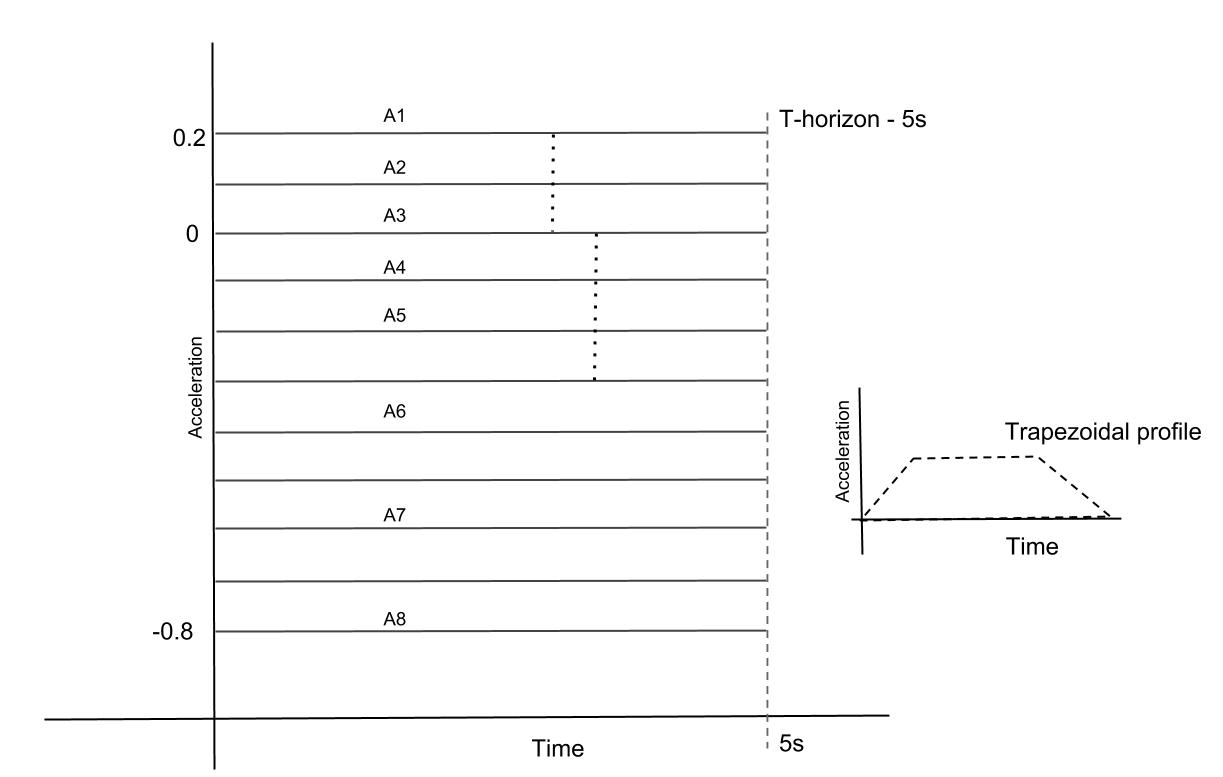
\includegraphics[width=0.8\textwidth]{Images/accelerations2.jpg}
    \caption{Different acceleration profiles a car can follow from current state. If target velocity is reached target acceleration is switched to zero as indicated by dotted lines.}
    \label{accelerations}
\end{figure}

 \begin{figure}
    \centering
    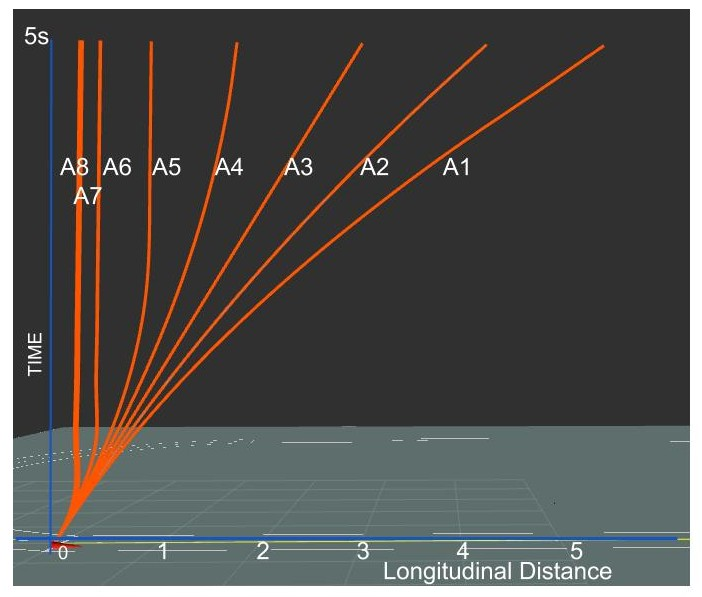
\includegraphics[width=0.8\textwidth]{Images/concept/distvstime2.jpg}
    \caption{Distance traversed vs time with accelerations A1-A8 from \ref{accelerations} in time horizon(5s), Initial position = (0,0) velocity = 0.6$ms^{-1}$, target velocity = 1.5 \& 0 $ms^{-1}$}
    \label{distances}
\end{figure}

 \begin{figure}
	\centering
	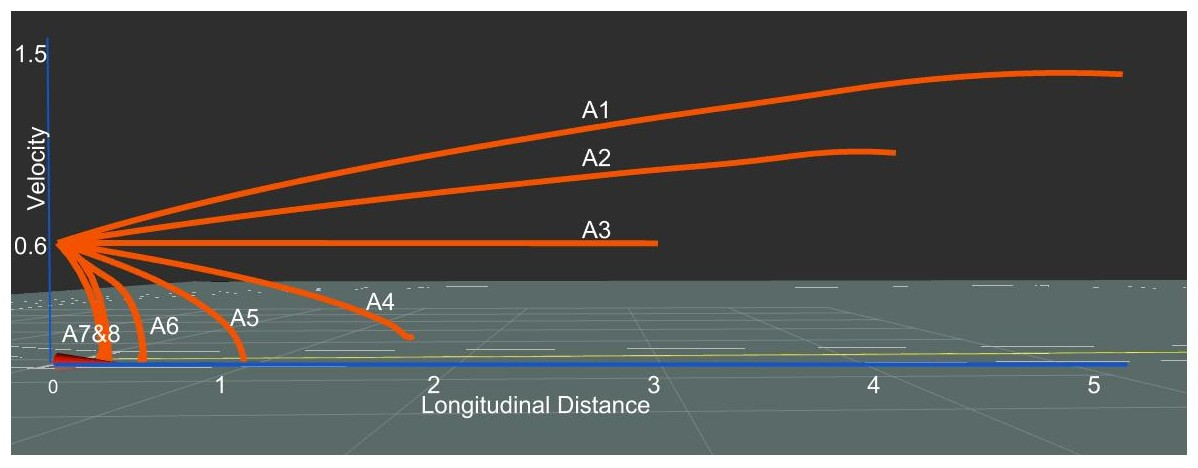
\includegraphics[width=0.8\textwidth]{Images/concept/distvsvel2.jpg}
	\caption{Distance traversed vs Velocity achieved with accelerations A1-A8 from \ref{accelerations} in time horizon(5s), Initial position = (0,0) velocity = 0.6$ms^{-1}$, target velocity = 1.5 \& 0 $ms^{-1}$}
	\label{velocities}
\end{figure}


\subsubsection{Lateral Planning}

Acceleration profiles discussed in \ref{lon_plan} solve the problem of longitudinal planning but to avoid obstacles the ego vehicle should also plan lateral (sideways) shifts in its trajectory. Similar to different accelerations, lateral shifts are sampled and combined along with acceleration samples to create final states. Lateral shifts can be mapped either as a function of time or distance traversed by ego vehicle. The research of Werling et al. \cite{werling_frenet} suggests that at lower speeds it is advantageous to map lateral shift as a function of distance and at a higher speed as a function of time. As this thesis is intended towards urban environments with limited speeds, lateral shift is mapped as a function of distance traversed. Lateral shift planning in this thesis is adopted from \cite{real_time_traj_plan_article}, which uses cubic splines and models lateral shift as a parameter of longitudinal distance as shown in equation \ref{lat_shift_one}. 

\begin{equation}
l(s) = c_0 + c_1s + c_2s^2 + c_3s^3
\label{lat_shift_one}
\end{equation}

The first and second derivative of the equation \ref{lat_shift_one} are equations for lateral velocity \ref{lat_vel} and acceleration \ref{lat_acc}.

\begin{equation}
    \frac{dl}{ds} = c_1 + 2c_2s + 3c_3s^2
\label{lat_vel}
\end{equation}


\begin{equation}
    \frac{d^2l}{d^2s} = 2c_2 + 6c_3s.
\label{lat_acc}    
\end{equation}

From the boundary conditions (0- initial state, f - final state), we have

\begin{equation}
l(s_0) = l_0 , l(s_f ) = l_f
\label{lat_boudary}
\end{equation}

The angle between the road frame and the vehicle is defined as $\theta(s)$, it can be derived from the first derivative of the lateral shift with respect to s. 

\begin{equation}
\theta(s) = arctan(\frac{dl}{ds})
\label{lat_veh_theta}
\end{equation}

To ensure the generated path follows current curvature and orientation of car and the final orientation is parallel to the road segment, following conditions should be satisfied.


\begin{equation}
\theta(s_0) = \theta_0 , \theta(s_f) = 0
\label{th_bundary}
\end{equation}

The figure \ref{lat_planning} indicates how the initial orientation will affect the shape of the trajectory. 

 \begin{figure}
    \centering
    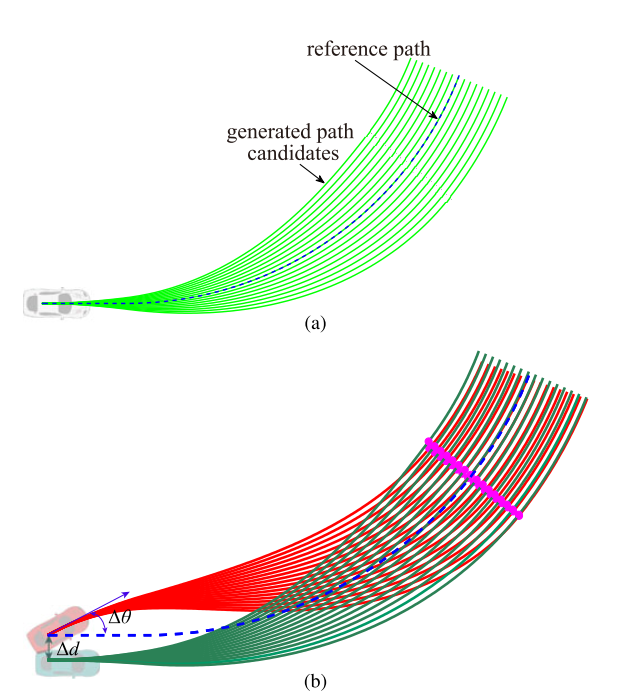
\includegraphics[width=0.8\textwidth]{Images/lateral_planning.png}
    \caption{Path candidates generation results. (a) Road parallel trajectories $l_0 = 0$ and $\theta_0 = 0$ (b) ego shifted with respect to center and driving at an angle $ 
l_0 = \Delta_d$ and $ \theta_0 = \Delta\theta$. \cite{real_time_traj_plan_article}}
    \label{lat_planning}
\end{figure}


The constants $ { c_0,c_1,c_2,c_3} $ in equation \ref{lat_shift_one} can be obtained by solving equations \ref{lat_vel} to \ref{th_bundary}.

The Figure \ref{searchspace} represents final search space by ego vehicle in XYT space, the density of this space can be increased by increasing the acceleration profiles and lateral samples. 

%Even the short changes in lateral shift create long trajectories that take $T_m$ time, to optimize and increase number of samples, trajectories that traverse lateral shifts in shorter horizon can be added. By ensuring that the samples from last selected trajectory are included in current sample set, smoother and consistent trajectories can be created

In summary, combining samples in acceleration and lateral shifts, multiple trajectories with different final states are created over the time horizon. In the next subsections how these trajectories are tested for collision with respect to static and dynamic obstacles is discussed. 

 \begin{figure}
	\centering
	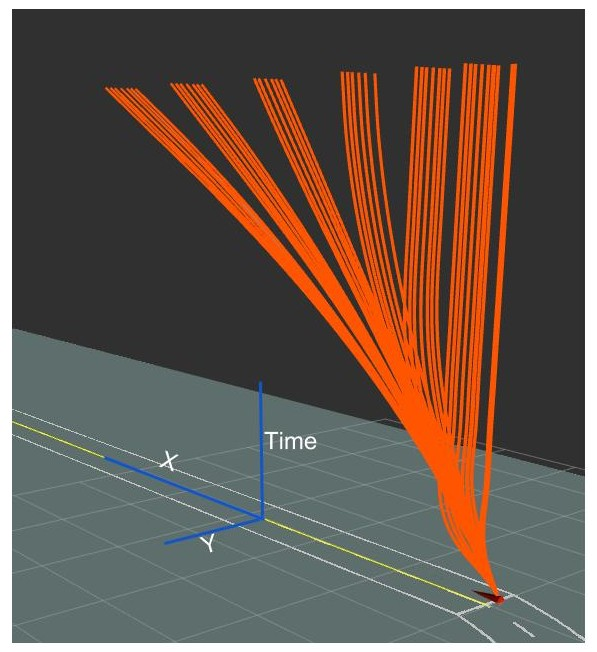
\includegraphics[width=0.8\textwidth]{Images/concept/searchspace2.jpg}
	\caption{Total search space in xyt}
	\label{searchspace}
\end{figure}


\subsection{Checking for Static Obstacles} \label{osbtacle_check_satic}
The primary objective of the motion planner is to derive a path that is collision free. The generated trajectories must be evaluated for collision or driving close to obstacles. There are various techniques for collision detection as discussed in the background study. This thesis developed a simple two-step collision checking technique for static obstacles. The obstacles are represented as rectangles (dilated enough to fit complete obstacle), and orientation of obstacles is divided into three categories, they are obstacles moving along, opposite or across the road. 

Initially for collision checking, obstacle coordinates are transformed into Frenet frame and represented by a length and width parallel to the road. In the first step, the trajectory in consideration is checked if it has a collision in longitudinal dimension (S coordinate) for the length of the obstacle with formula \ref{intersection_reg}. As shown in Figure \ref{static_check} trajectories T0, T1 intersect in S-dimension for obstacle O1 and not for obstacle O2. The next step is to find this intersection region, I1 to I2 in Figure \ref{static_check} represent the S-dimension intersection, the values are dilated for safety. In final it is checked whether from I1 to I2 there is a collision in lateral dimension(d) for trajectory and obstacle. For all points between I1 and I2, the lateral distance between trajectory and obstacle must always be larger than safety value as described in \ref{static_obst_safety_dist}. As the function representing lateral motion is a continuous function, it is sufficient to check for collision at the start and end of the intersection interval and at critical points (where derivative of the function is zero or does not exist) if they fall in the intersection region. If the distance at any of these points is less than the minimum required or difference vector has different sign then there is a collision. Appendix \ref{static_obst_appendix} details further on sufficiency to check only at critical points and borders. 

\begin{equation}\label{intersection_reg}
\begin{aligned}
intersection = [max(min(obst_s.begin(),obst_s.end()),path.front()),\\ min(max(obst_s.begin(),obst_s.end()),path.back())]
\end{aligned}
\end{equation}

If $(intersection[1]<intersection[0])$  then there is no intersection in the two paths. 


\begin{equation}
    |d\textsubscript{ego} - d\textsubscript{obst}| > car\_width/2 + obstacle\_width/2 + safety\_margin
    \label{static_obst_safety_dist}
\end{equation}

It is representative from figure \ref{static_check} that the trajectory T1 has collision and trajectory T0 has no collision. Different costs can be added based on how close the ego vehicle is with respect to the static obstacle.  

 \begin{figure}
    \centering
    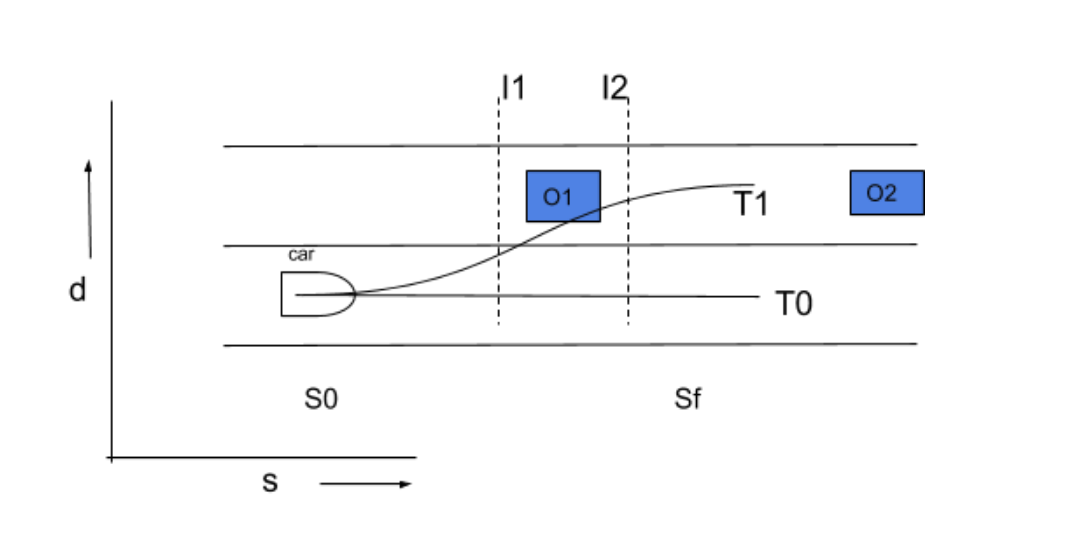
\includegraphics[width=0.8\textwidth]{Images/static_check.png}
    \caption{Collision check for static obstacles, I1-I2 represent collision region in S-dimension, in this region T1 intersects with trajectory and T0 is collision free.}
    \label{static_check}
\end{figure}



\subsection{Checking for Dynamic Obstacles} \label{obstacle_check_dynamic}

In dynamic environments such as cities, it is vital to plan collision-free trajectories by predicting the state of other obstacles. Predicting the future behaviour of obstacles is a challenging part of urban driving, various approaches used are described in subsection \ref{traj_eval}. This thesis models dynamic obstacles as squares continuing with their current speed in their detected lane/lateral position for planning duration similar to \cite{unit_A_star} or moving in opposite direction or moving across the lane based on the angle between the obstacle and road. This assumption can be justified by the fact that the trajectories are re-evaluated at high frequencies and any changes in obstacles lateral distance, orientation or speed will be evaluated in next cycle thus keeping the vehicle safe from the collision. 

The collision check for dynamic obstacles has one extra check-in time dimension as compared to checking for static obstacles, it is inspired by forbidden regions calculation as discussed in \cite{graff_thesis}. In step one the intersection in S coordinate for obstacle and ego vehicle is found, here the length of the obstacle is dilated over the distance travelled by obstacle as represented by dotted line ahead of the obstacle in figure \ref{dynamic_check}. If there is a collision in S dimension, then the collision between ego vehicle and obstacle in lateral dimension (D) in the intersection region I1 to I2 is tested in a similar way to static obstacle collision check. If there is a collision in D dimension, then the corresponding S dimension where there is collision is found, represented with J1-J2 in figure \ref{dynamic_check} (generally this will be shorter than I1 - I2). For the range J1-J2, it is checked if they collide in time also, i.e., if they reach the same location in same time, a buffer time is added to be safe. As per instructions for safe driving it is required for the car to maintain a minimum time gap of 2 seconds with the vehicle ahead. There are more formal methods \cite{mobile_eye_safety_distance} on safety distances for self-driving cars. This thesis implements a simple 2-second rule to safety, and this is a tunable parameter which can be used to increase driving aggression. Figure \ref{dynamic_close1} indicates a similar situation for the collision in time dimension for scenario presented in Figure \ref{dynamic_check} with the difference that the obstacle is in a different lane.

 \begin{figure}
	\centering
	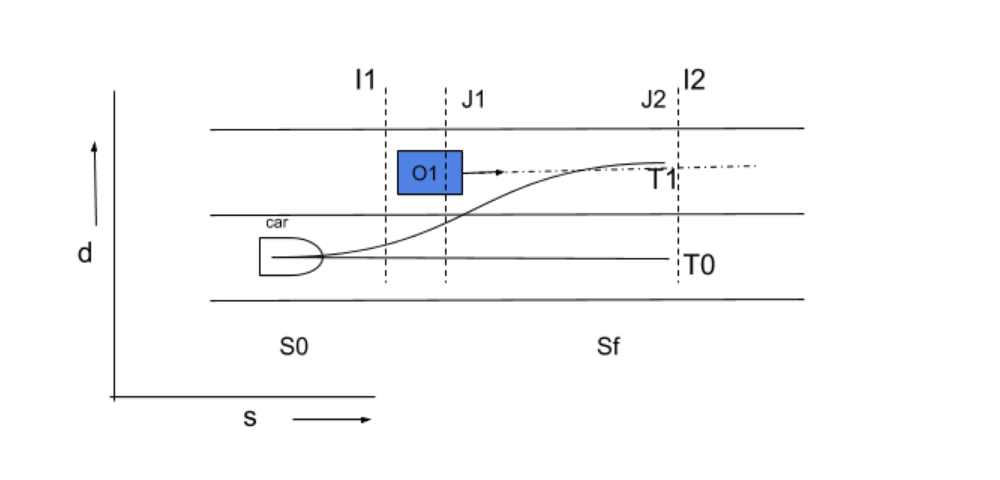
\includegraphics[width=0.8\textwidth]{Images/dynamic_check.png}
	\caption{Collision check for Dynamic obstacles, I1-I2 represent collision in S-dimension, J1-J2 indicate collision in S and D dimension.}
	\label{dynamic_check}
\end{figure}

To check collision in time dimension, time difference between the ego vehicle and the obstacle at the S dimension intersection borders is tested as shown in figure \ref{dynamic_obst_all}. If the gap is larger than 2 seconds at all the times and doesn't change sign then there is no collision, Figure \ref{dynamic_obst_all} a) b) present situation where the time to the collision between ego vehicle and obstacle reduces but there is no collision. If the time difference between ego vehicle and the obstacle has an opposite sign at the start and end of the intersection region, then it detected as a collision. As difference indicates time to collision, and as time and distance are continuous. A change in sign in time difference demonstrates that in between at some point there was a collision (difference = 0). Figure \ref{dynamic_obst_all} c) and d) present a situation where the projected trajectory of the ego vehicle will collide with a dynamic obstacle. Figures \ref{dynamic_obst_all} e) represent a case where the planned trajectory of ego vehicle collides with obstacle moving in opposite direction and Figure \ref{dynamic_obst_all} f) represents where the ego vehicles projected trajectory will not collide the vehicle in reverse lane.


\begin{figure}
	\centering
	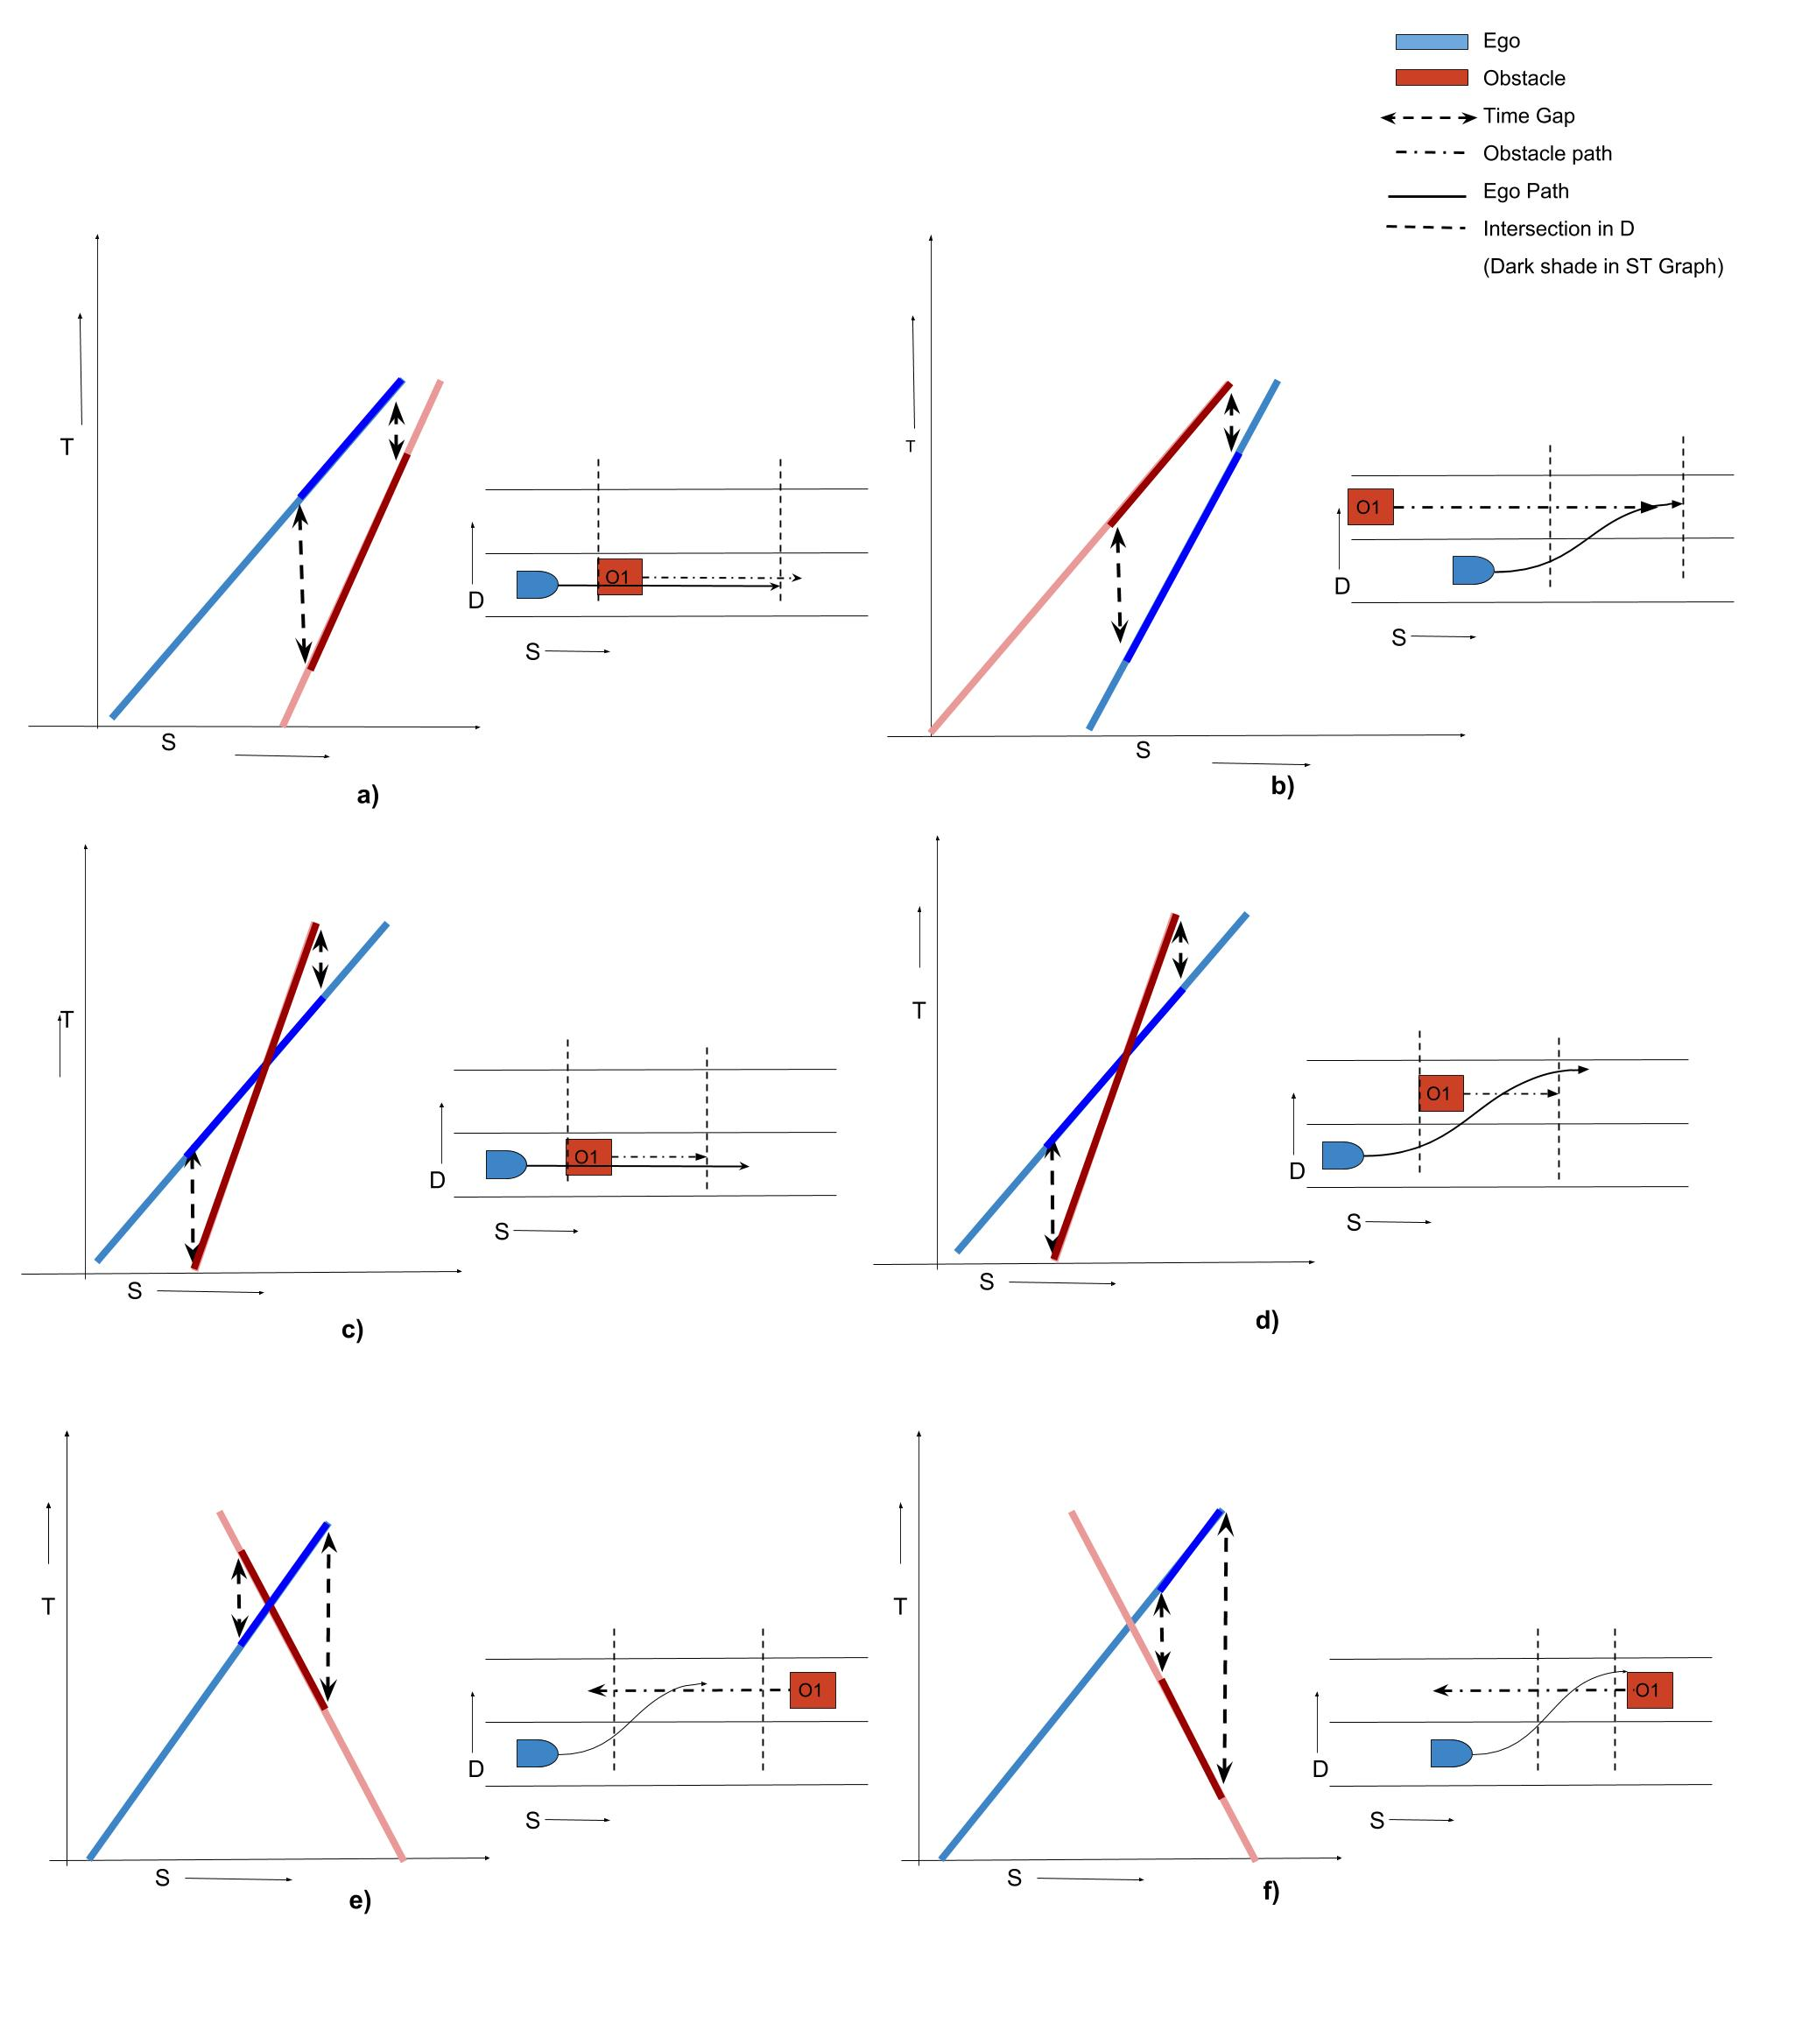
\includegraphics[width=1.1\textwidth]{Images/concept/dynamic_collision_lines.jpg}
	\caption{a),b) describe situations where ego vehicle's projected trajectory is close to obstacle ahead and behind respectively, but not colliding. \newline 
		c),d) describe situations where ego vehicle's projected trajectory collides with obstacles ahead and obstacle in next lane respectively. \newline
		e) describes situation in which ego vehicle's projected trajectory collides with obstacle moving in opposite direction and f) describes situation where it will not collide. 
	}
	\label{dynamic_obst_all}
\end{figure}

The method discussed till now represents the ego vehicle and the obstacle as points moving in space-time, but both of them have lengths. Thus, the time at the beginning and end of intersection region should consider the length of these objects, i.e., time for ego or obstacle to cross this point should be considered. As presented in Figure \ref{dynamic_widths}, time gap at the start of intersection is the minimum of the four-time gaps formed between front of the ego and front of the obstacle, front of the ego and back of obstacle, back of the ego and front of the obstacle, back of the ego and back of the obstacle to cross the beginning of the intersection region. Similarly, minimum of these four-time gaps are considered to find the time gap at the end of the intersection.

\begin{figure}
	\centering
	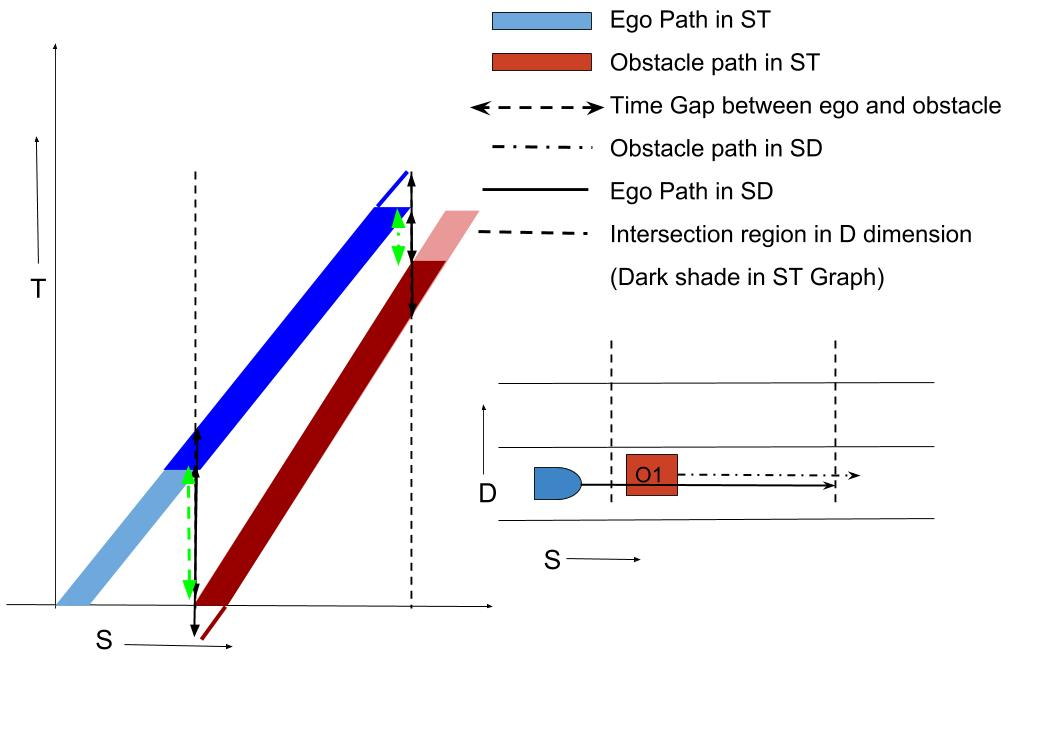
\includegraphics[width=0.8\textwidth]{Images/concept/dynamic_obst_widths.jpg}
	\caption{Collision checking by considering the length of the car and the obstacle. Time gap at the intersection is the gap between the front of ego and back of ego to cross that point, represented by green arrowed lines.}
	\label{dynamic_widths}
\end{figure}

Dynamic obstacle moving laterally across the road are represented as static obstacle occupying the length of the road. Thus, if there is a pedestrian crossing the road, the trajectory is considered to be in the collision if there is a collision in S dimension and there will anyways be a collision in D dimension due to dilation of the pedestrian width to the width of the road and no time dimension is checked. This could, however, be improved by checking the direction of walking and also predicting the time to cross the road to check for collision. 

In the Figure \ref{dynamic_obst_all} motion of the ego vehicle is approximated with linear velocity, but in reality, this is not the case, ego vehicle follows a parabolic path with respect to time because of acceleration and deceleration. Figure \ref{dynamic_approx} presents a scenario where the ego vehicle with $0.1ms^{-1}$ velocity is accelerated at $0.2ms^{-2}$ represented with a blue line and an obstacle moving at $0.6ms^{-1}$ represented by a red line. In this situation at the start and end of the intersection region time difference between the ego and obstacle is positive (green lines) but there is a collision in the middle of the path. The algorithm mentioned above could not detect this collision. There are two ways to mitigate this effect. One is to have a substantial enough buffer time which covers the non-linearities caused by the parabolic path. In the Figure \ref{dynamic_obst_all} orange line between the linear approximation path (Yellow line) and ego path (blue line) represents the maximum difference caused by non-linearity. It is around $0.8s$, and this thesis employs a two-second rule to detect a collision. Thus, if the time difference between the ego and the obstacle intersection region is greater than two seconds at borders, then there is no collision between the two, at some point in the middle they may come close but will not collide. Appendix \ref{dynamic_obst_appendix} provides proof about this hypothesis being correct. Another way to mitigate this issue is to check at multiple points in intersection region to determine collision. The second method can be employed when aggressive driving is needed, and distance to obstacles is kept to a minimum.

%Collision checking in dynamic environments approximated as the path from start to end with linear velocity, in reality, this is not true, and there will be acceleration and deceleration by ego vehicle. Figure \ref{dynamic_approx} presents scenario where the ego vehicle with $0.1ms^{-1}$ velocity is accelerated at $0.4ms^{-2}$, the corresponding approximated line for 5s if line with uniform velocity of $1.1ms^{-1}$. For this approximation to be safe the time difference between the original path and the approximated line should never be greater than $2s$, the maximum time difference as presented by the black line is $0.8s$. The difference is affected mainly by the acceleration and deceleration values with higher values causing a higher shift. Due to limits on maximum speed, acceleration and minimum speed of zero, the approximation holds good for the 5s horizon with a maximum observed difference of 0.8s to approximation. To reduce the safety margin to less than 0.5s, simply adding checks at every second instead of the start and end are sufficient. 

\todo{Compared to simulation based methods this method is faster to implement and works for different velocities easily, where to write this? - evaluation }

\iffalse %commented all the 3 individual sub pictures and used one picture together
\begin{figure}
	\centering
	\begin{subfigure}{.51\textwidth}
		\centering
		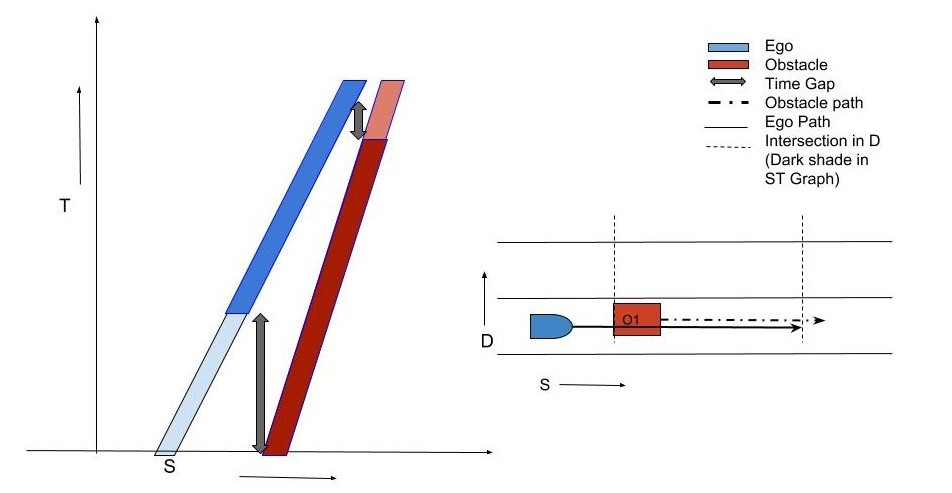
\includegraphics[width=1.0\textwidth]{Images/concept/dynamic_close1.jpg}
		\caption{Ego vehicle projected trajectory getting close to slow moving obstacle ahead}
		\label{dynamic_close1}
	\end{subfigure}%
	\begin{subfigure}{.49\textwidth}
		\centering
		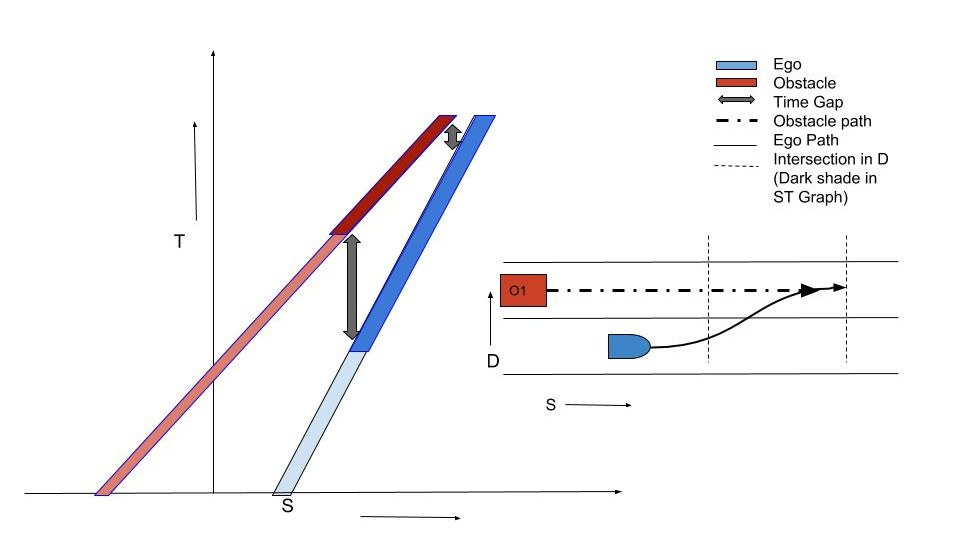
\includegraphics[width=1.0\textwidth]{Images/concept/dynamic_close2.jpg}
		\caption{Ego vehicle projected trajectory getting close to a fast moving dynamic obstacle in next lane while performing a lane change}
		\label{dynamic_close2}
	\end{subfigure}
	\caption{Ego vehicle getting close to dynamic obstacale but not colliding}
	\label{dynamic_close}
\end{figure}


\begin{figure}
	\centering
	\begin{subfigure}{.515\textwidth}
		\centering
		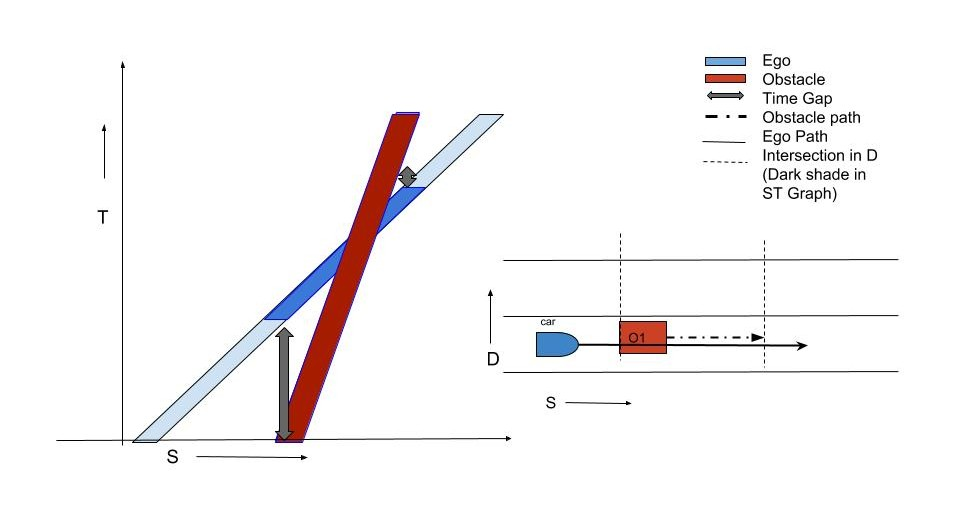
\includegraphics[width=1.0\textwidth]{Images/concept/dynamic_collison.jpg}
		\caption{Ego vehicle projected trajectory colliding with obstacle ahead}
		\label{dynamic_collision1}
	\end{subfigure}%
	\begin{subfigure}{.485\textwidth}
		\centering
		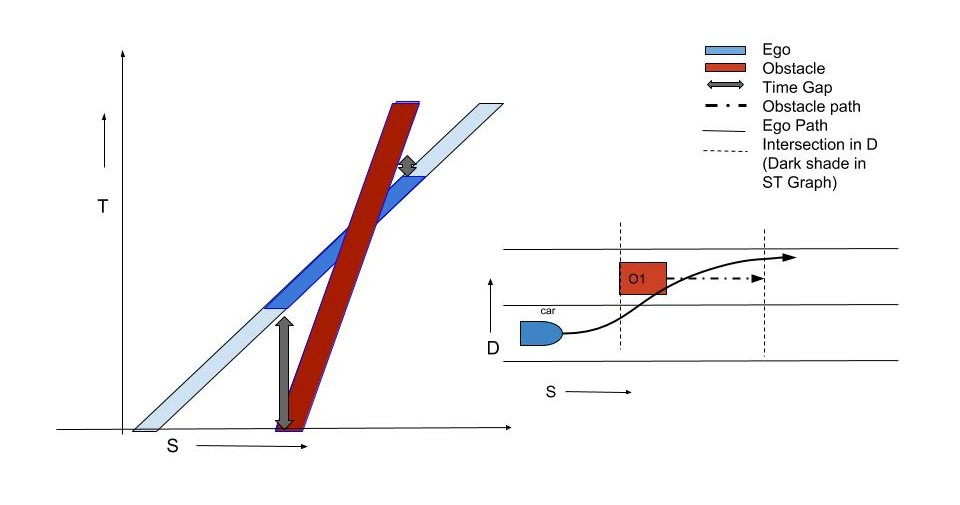
\includegraphics[width=1.0\textwidth]{Images/concept/dynamic_collison2.jpg}
		\caption{Ego vehicle projected trajectory colliding with obstacle ahead while performing lane change}
		\label{dynamic_collision2}
	\end{subfigure}
	\caption{Ego vehicle projected trajectory colliding with obstacle in future.}
	\label{dynamic_collision}
\end{figure}

\begin{figure}
	\centering
	\begin{subfigure}{.515\textwidth}
		\centering
		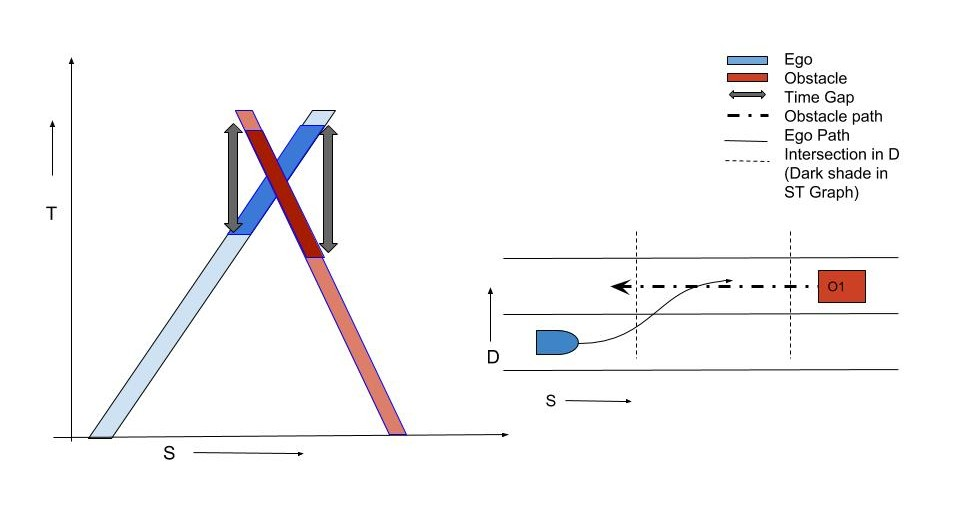
\includegraphics[width=1.0\textwidth]{Images/concept/dynamic_opposite_collision.jpg}
		\caption{Ego vehicle projected trajectory colliding with obstacle moving in opposite direction}
		\label{dynamic_opp1}
	\end{subfigure}%
	\begin{subfigure}{.485\textwidth}
		\centering
		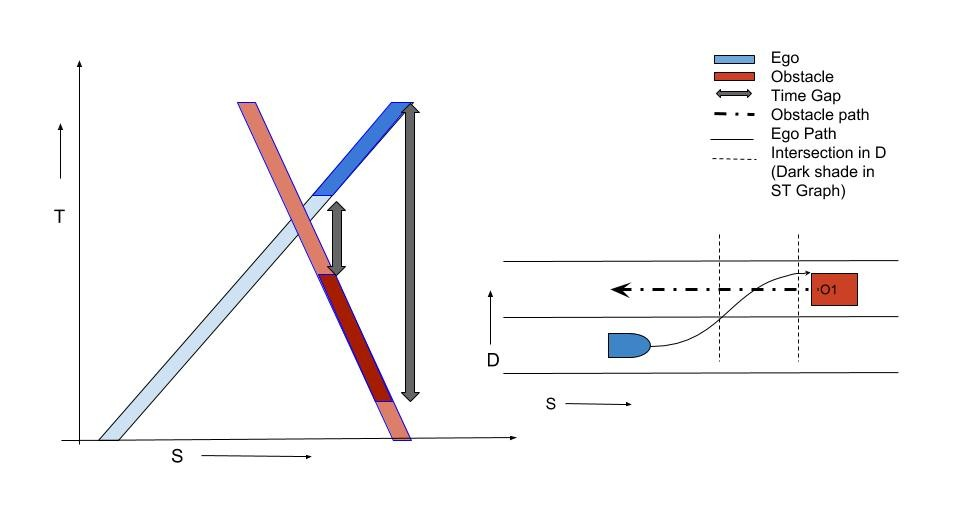
\includegraphics[width=1.0\textwidth]{Images/concept/dynamic_opposite_nocollision.jpg}
		\caption{Ego vehicle projected trajectory performing a lane change and not colliding with obstacle in next lane}
		\label{dynamic_opp2}
	\end{subfigure}
	\caption{Ego vehicles interaction with }
	\label{dynamic_opp}
\end{figure}
\fi



 \begin{figure}
	\centering
	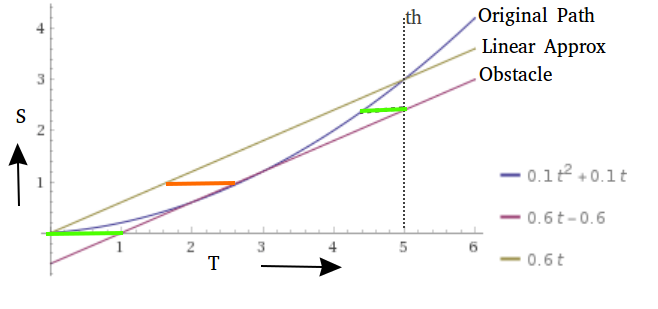
\includegraphics[width=0.8\textwidth]{Images/concept/dynamic_obstacle_new.png}
	\caption{Parabolic Path and collision checking}
	\label{dynamic_approx}
\end{figure}

%\begin{figure}
%    \centering
%    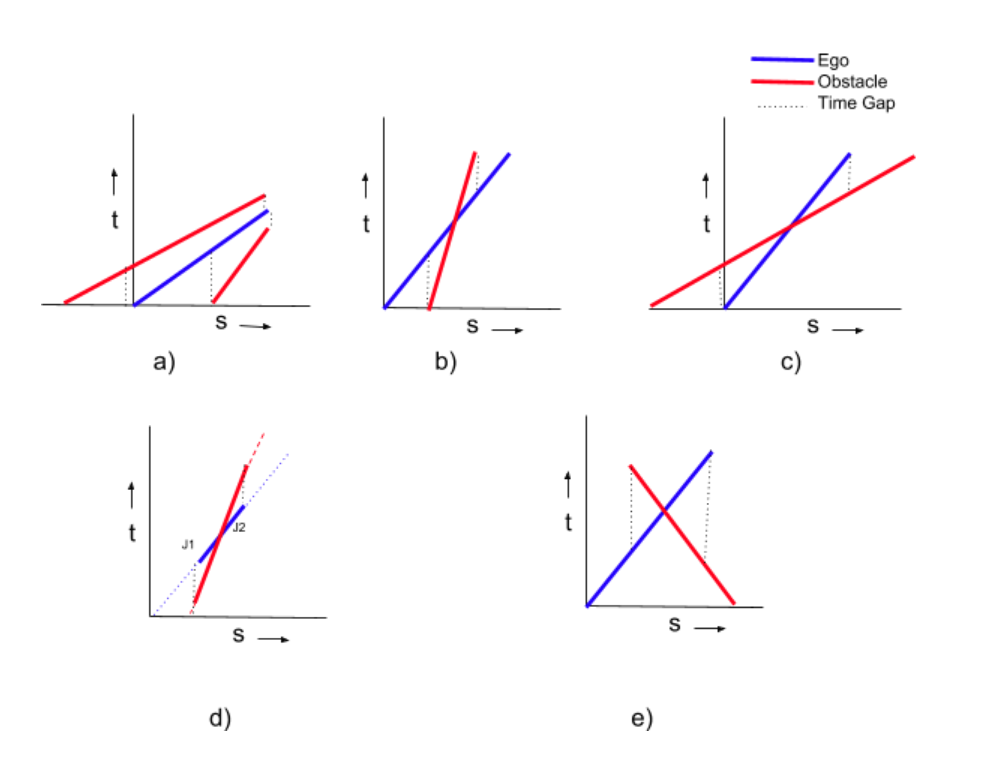
\includegraphics[width=0.8\textwidth]{Images/dynamic_Check_time.png}
%    \caption{Collision check in space Time a) indicates obstacles getting close to the ego vehicle but not colliding. b) Ego vehicle hits the slow moving obstacle ahead. c) Ego vehicle is hit by fast moving obstacle behind - Situation during unchecked lane change by ego vehicle }
%    \label{dynamic_time_check}
%\end{figure}



%Dynamic obstacles are assumed to continue in the lane they are detected and if an obstacle is found across two lanes then it is assumed to be performing lane change and modelled as two dynamic obstacles moving straight in both lanes to overcome uncertainty.


%The collision check dynamic obstacles is performed in two stages, in first stages bounding boxes are drawn across the length of the trajectory of both the ego vehicle and the dynamic obstacle across time T. If the bounding boxes intersect then the second stage of collision check is invoked. In this step, both the dynamic obstacle and ego vehicle are moved in unit steps of time and checked for collision. As per the earlier assumption, dynamic obstacles tend to move in the lane they are detected thus to make the collision check simple, 3 lines are drawn across the corners and centre of the vehicle. The lines are extended for unit time and if the 3 lines intersect with the ego vehicle bounding square then there is a collision. The figure \ref{dynamic_obstacle} details further about the collision check.
%\todo{(The representation is not correct in figure, take the representation from the cited pages for further ease)}
%\todo{bounding boxes - Autonomous Driving in Dynamic Environments}
%\todo{Cite this paper for $3$ line collision-  An RRT-based Navigation Approach for Mobile Robots and Automated Vehicles-RRT*\_. pdf}




\subsection{Cost Functions and Trajectory Selection} \label{traj_Selection}
Selection of final trajectory is based on the different costs associated with it, and costs can be static and dynamic. Static costs are known before trajectory creation and dynamic costs are known after the trajectory is created and evaluated. There is wide research on different costs involved in trajectory selection as discussed in section \ref{traj_eval}

This thesis implements a simple cost function as represented in \ref{cost_eqn}; explicit smoothness costs are not considered as the target validation platform is a model car with no humans inside and limitations of the model car to track a fine trajectory. 
\begin{equation}
initial_cost = |V_a - V_t| + |a_t| + | (d_t - d_e)*k1 | + | (d_p - d_e)*k2 |\
\label{cost_eqn}
\end{equation}
$V_a$ - velocity achieved by trajectory.
$V_t$ - Target Velocity.
$a_t$ - Target Acceleration.
$d_t$ - Target lateral distance.
$d_e$ - Trajectory lateral distance.
$d_p$ - Previous target lateral for trajectory.
$k_1,k_2$ - Factors to adjust weights, currently used at 0.8 and 0.2

The velocity and acceleration terms in cost function \ref{cost_eqn} promote higher accelerations if the target and current velocity difference are higher and lower accelerations if the difference is low. The next lateral terms promote the trajectories that are closer to the target lateral distance and also close to the previous selection thus limiting the shifts in path selection and maintaining continuity. The initial cost of the previous path is kept to zero to promote ego to follow old path if there is no collision. 

The final cost for trajectory selection is the sum of the initial cost, collision detection cost for trajectory and horizon cost as mentioned in equation \ref{final_cost}. Horizon cost is added to samples if the created trajectory crosses the destination thus promoting the trajectories that stop at the goal. 

\begin{equation}
final_cost = initial_cost + collision_cost + horizon_cost
\label{final_cost}
\end{equation}

Initially, all the sampled trajectories are assigned the costs based on the cost function \ref{cost_eqn} and sorted, then the trajectory with the lowest cost is evaluated and the final cost is calculated as per equation \ref{final_cost}. The list is sorted again and evaluated till the top of the list has the lowest cost, and the trajectory is evaluated. Thus the trajectories with initial assumption are validated, and best one is chosen in the end. 

\subsection{Velocity Planning}
Velocity planning is an important aspect of the planer, in general, behavioural layer defines the target velocity based on speed regulation, other traffic participants, required behaviour, road condition etc. In this thesis, a simple approach of velocity limiting is used based on road curvature to limit lateral accelerations. Max velocity  V\textsubscript{max} is calculated based on the equation \ref{max_vel}. 

\begin{equation}
    V\textsubscript{max} = min(\sqrt{Acc\textsubscript{MaxLat} / |k(s)|} , V\textsubscript{limit})
\label{max_vel}
\end{equation}
$V\textsubscript{limit}$ - Velocity limit mentioned in road network,
$Acc\textsubscript{MaxLat}$ - Maximum Lateral acceleration(based on comfort and vehicle dynamics),
$k(s)$ - Road curvature.

\section{Trajectory Follower} \label{traj_follower}

The controller for following the trajectory is adopted from Made In Germany (MIG) autonomous vehicle. The work \cite{mig_controller} details further on how the trajectory is decomposed into steering and speed commands. 

\chapter{Implementation}
\label{implementation}
Check if this chapter is needed, 

Here I can write mostly about how the state machine is implemented to choose profiles

How the collision check is implemented

Further details on how these trajectories are converted to x,y coordinates used by the trajectory follower and the constraints in implementation for model car will be discussed in

How costs are added


How the messages flow, 


Which messages are received, which messages to be 

I would prefer to finish this in Planning Chapter 

speak about splines, how the state machine works, write a flowchart etc

how the conversion happens and where it happens etc etc
\include{Chapters/Discussion}
\chapter{Evaluation}
\label{evaluation}
In previous chapters detailed working of the planning algorithm has been discussed, this chapter discusses the evaluation criteria and results in detail. Various concepts discussed previously will be examined here through a series of experiments reflecting real life driving scenarios. This chapter is organized as follows: Section \ref{experiments} discusses systematic evaluation of the planner by exposing it to various scenarios equivalent to on-road driving conditions. The next section \ref{criteria_based_eval} discusses a criteria based evaluation for the planner similar to any algorithm in the form of feasibility, optimality, completeness, run-time etc.

\section{Experiments}\label{experiments}
Due to time and resource constraint most of the experiments to evaluate the planner are performed on simulator. The test cases involve finding a collision free path with obstruction in driving lane, avoiding slow moving traffic, merging into ongoing traffic, lane changes etc. The following subsections detail further on each experiment. 

\subsection{Lane blocked}
In driving scenario  \ref{lane_blocked_1}, driving lane is blocked by a static obstacle and a slow moving obstacle is in the next lane, here ego vehicle drives slowly till it finds enough room in the next lane, once obstacle is avoided the robot continues to shift into intended lane and drives with increasing speed. 

\begin{figure}[h]
    \centering
    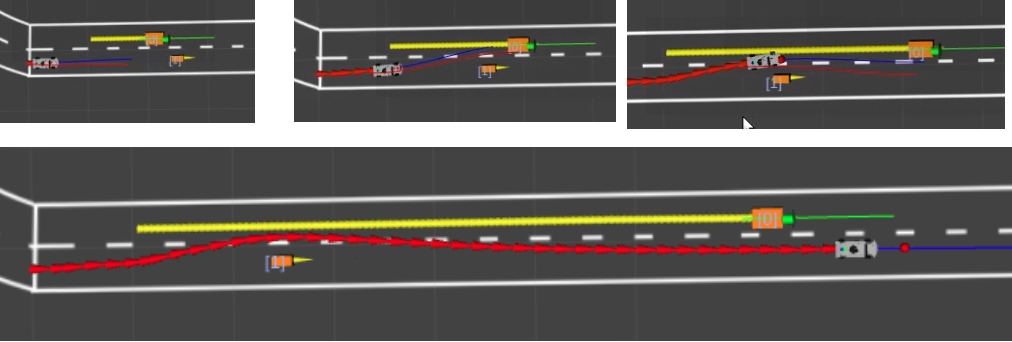
\includegraphics[width=0.8\textwidth]{Images/evaluation/lane_blocked1.jpg}
    \caption{Driving Lane Blocked}
    \label{lane_blocked_1}
\end{figure}

\subsection{Slow Moving Traffic}
In situation 1 presented in Figure \ref{slow_moving_1} ego vehicle starts changing into left lane once a slow moving obstacle is encountered, once the obstacle is passed it starts driving into right lane again. In situation 2 presented in Figure \ref{slow_moving_2} there are two slow moving obstacles ahead, once the ego vehicle overtakes the initial obstacle it shifts to original lane as intended but it encounters the second slow moving obstacle and shifts to left lane again. This behavior is caused because of locally optimal cost functions driving the ego vehicle into intended lane without knowledge of long term planning information. A behavioral layer with longer scenario analysis horizon will result in better path selection.
\begin{figure}[h]
    \centering
    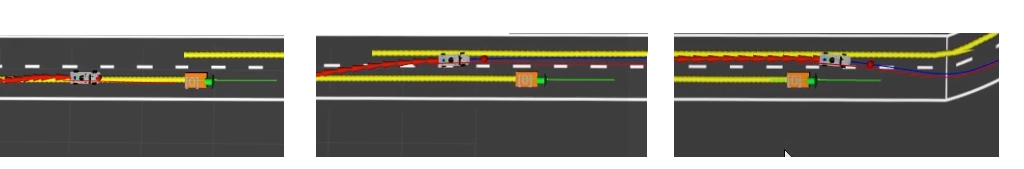
\includegraphics[width=0.8\textwidth]{Images/evaluation/slow_moving1.jpg}
    \caption{Slow Moving Traffic Situation 1}
    \label{slow_moving_1}
\end{figure}

\begin{figure}[h]
    \centering
    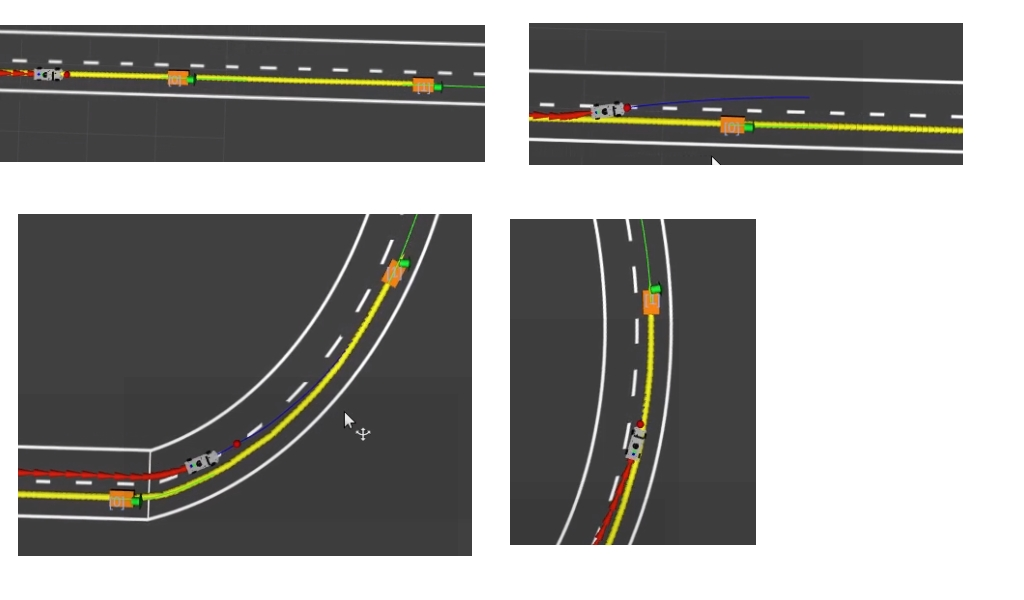
\includegraphics[width=0.8\textwidth]{Images/evaluation/slow_moving2.jpg}
    \caption{Slow Moving Traffic Situation 2}
    \label{slow_moving_2}
\end{figure}

\subsection{Merging into traffic}

In scenario presented in Figure \ref{merging1}, lane changing is requested to merge into the traffic in left lane. Here ego vehicle speed is $1ms^(-1)$ and obstacle speed is $0.6m^(-1)$. Initially lane change does not occur as cost functions are tuned to maintain speed over maintaining required lane. As the vehicle enters the curve, target driving speed is reduced and the vehicle merges into the traffic in left lane. Depending on which portion of the lane the ego vehicle is in i.e, near intersections or exits target lane should have higher priority over maintaining speed and during rest of the regions target speed should be of higher priority to reach destination quickly. Cost functions implemented in this thesis provide flexibility in tuning behavior of the ego vehicle. 

\begin{figure}[h]
    \centering
    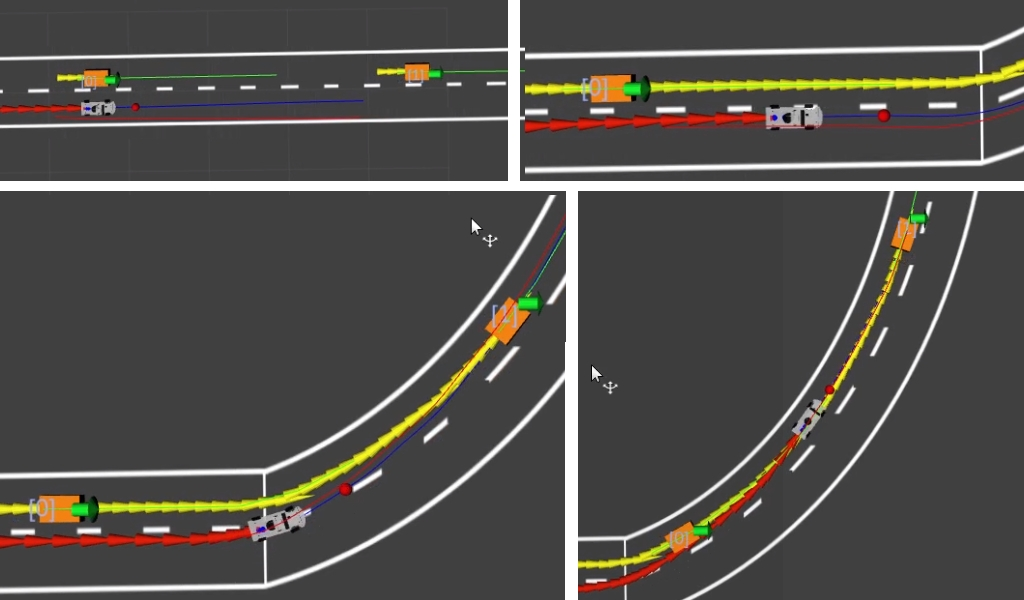
\includegraphics[width=0.8\textwidth]{Images/evaluation/merging1.jpg}
    \caption{Merging into Traffic}
    \label{merging1}
\end{figure}

\subsection{Merging into next lane with opposite traffic}

In scenario presented in Figure \ref{series_obstacles} driving lane is blocked by a series of obstacles and the left lane is occupied by a moving obstacle. Ego vehicle starts slow in the driving lane and waits till the obstacle is passed in the left lane and starts driving forward. 
\begin{figure}[h]
    \centering
    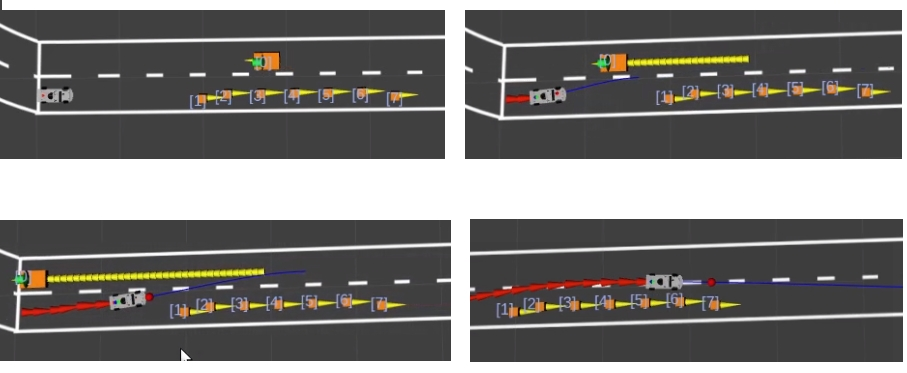
\includegraphics[width=0.8\textwidth]{Images/evaluation/series_lane_blocked1.jpg}
    \caption{Lane blocked by series of static obstacles and vehicle in next lane driving opposite}
    \label{series_obstacles}
\end{figure}

This situation may lead to ego vehicle getting stuck in middle of the road. If driving speed of ego vehicle is low, temporal horizon limits ego vehicles lookahead distance into future. If a fast moving obstacle in left lane not visible in 7 seconds(5 planning and 2s of safety) of temporal horizon then the ego vehicle starts lane change and if there is time to abort it will abort and if not the ego vehicle will stop in middle of the lane due to no path ahead, if the obstacle proceeds without stopping for ego vehicle. This can be avoided by a behavioral layer with longer spatial scenario analysis horizon. As the planner discussed in this thesis is not created for controlling the vehicle to drive backwards, a different planner equivalent to off road planner must be used.  


\subsection{Road Blocked or Pedestrian Ahead}

In scenario presented in Figure \ref{road_blocked}, road is blocked by a series of static obstacles, the vehicle enters empty left lane, slows down and finally stops when it cannot find route ahead. 

\begin{figure}[h]
    \centering
    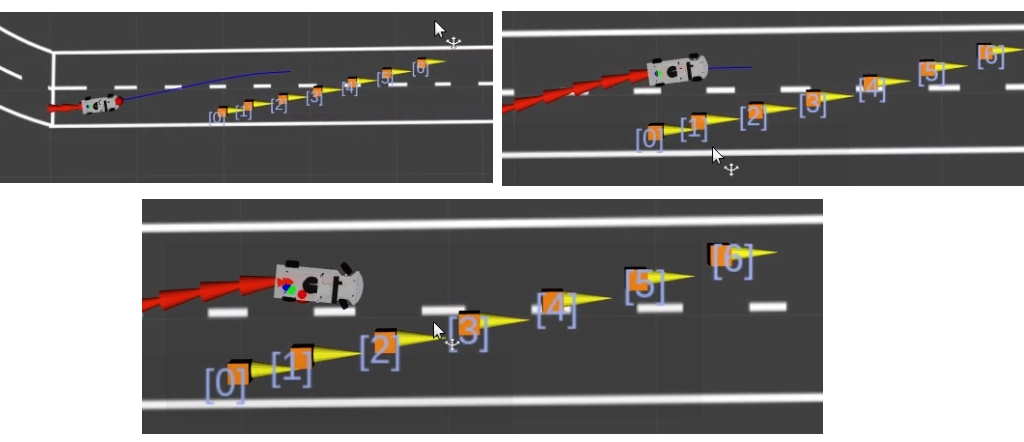
\includegraphics[width=1.0\textwidth]{Images/evaluation/road_blocked1.jpg}
    \caption{Road Blocked by series of obstacles}
    \label{road_blocked}
\end{figure}

A pedestrian on road is considered similar to a road blocking, in this case as shown in Figure \ref{pedestrian_ahead} the ego vehicle initially drives at full speed, then the vehicle slows down(shorter blue line representing a slower speed) and the robot finally comes to halt few meters ahead of the pedestrian. This is a tunable parameter and currently at maximum value for safety. 

\begin{figure}[h]
    \centering
    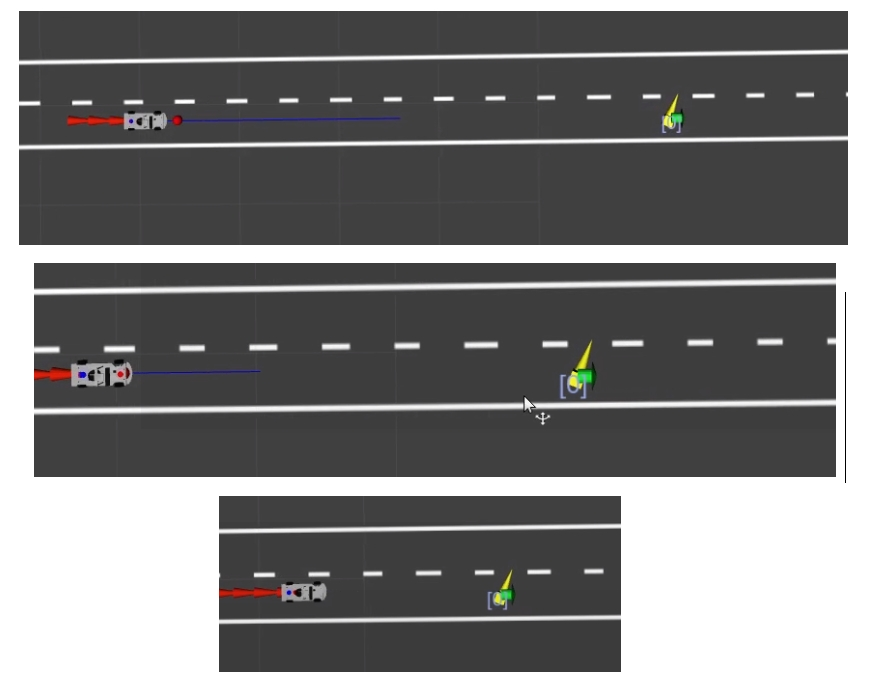
\includegraphics[width=0.8\textwidth]{Images/evaluation/pedestrian_ahead.jpg}
    \caption{Pedestrian Ahead on Road}
    \label{pedestrian_ahead}
\end{figure}

\subsection{Dynamic Obstacles - other vehicles}
The main objective of the planner is to adjust to the sudden changes in the environment caused by the dynamic obstacles in surroundings, here two sub scenarios are described where the ego vehicle has to react to sudden breaking of vehicles ahead. 

In scenario presented in Figure \ref{dynamic_1}, there are two situations. In situation 1 the car aborts a lane change when the slow moving dynamic obstacle in left lane is detected, then once the dynamic obstacle is passed the vehicle shifts to left lane to avoid the stopped dynamic obstacle in driving lane. This situation is similar when a vehicle ahead stops to drop off a passenger or waiting for parking spot. In situation 2, the car doesn't choose lane change initially and slows down till it finds enough room in left lane to drive ahead of the stopped dynamic obstacle. 

\begin{figure}[h]
    \centering
    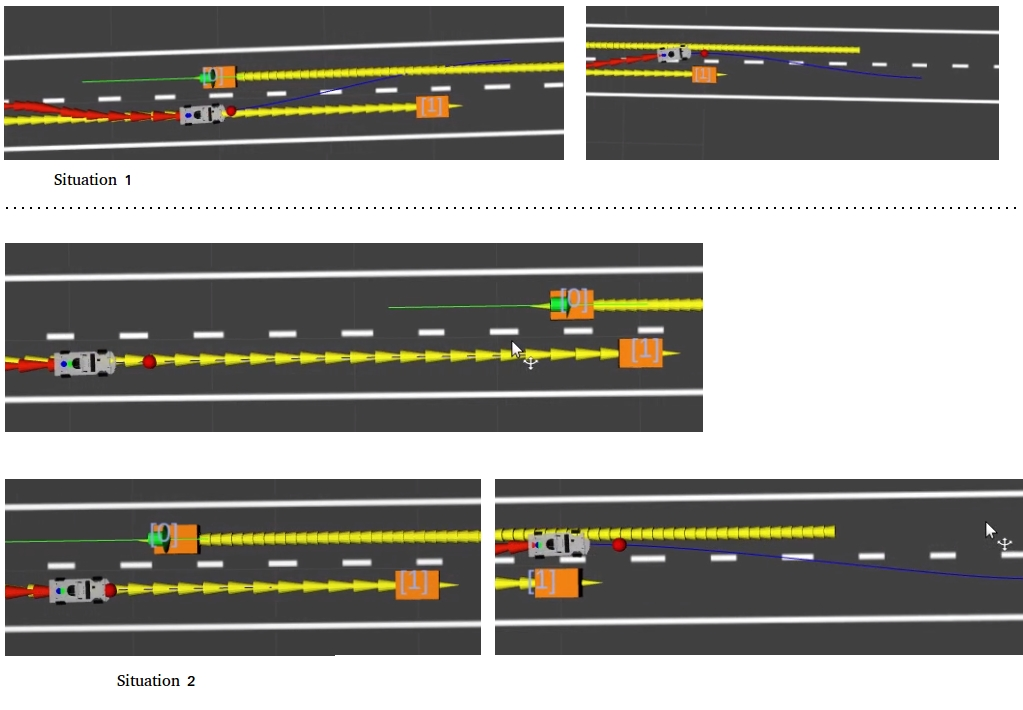
\includegraphics[width=0.8\textwidth]{Images/evaluation/dynamic_ahead_breaking1.jpg}
    \caption{Dynamic Obstacle Ahead stops in middle of road}
    \label{dynamic_1}
\end{figure}

In scenario presented in Figure \ref{dynamic_2} there are two situations with different thresholds for safety, in situation 1 a safe 2s+ distance to obstacles ahead is chosen, here the ego vehicle stays far away from the vehicles ahead and when it stops it stops relatively farther from the vehicles ahead. In situation 2, the threshold has been adjusted to 0.5s leading to a aggressive behavior of ego vehicle. The ego vehicle drives closer to the obstacles ahead and when the dynamic obstacles ahead stop suddenly, distance between the ego vehicle and the obstacles ahead is very narrow.   
\begin{figure}[h]
    \centering
    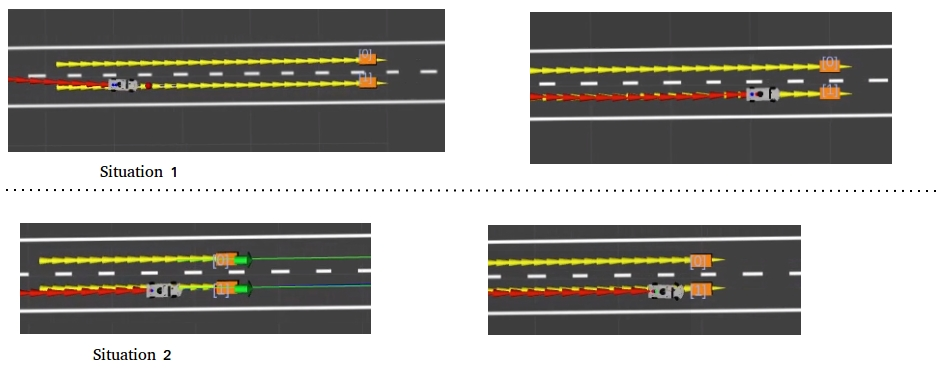
\includegraphics[width=0.8\textwidth]{Images/evaluation/dynamic_ahead_breaking2.jpg}
    \caption{Two Dynamic Obstacles ahead stop suddenly}
    \label{dynamic_2}
\end{figure}

%\subsection{Avoiding Static Obstacles}
%\subsection{Avoiding Dynamic Obstacles}
%\subsection{Avoiding Pedestrians}
%\subsection{Lane Changing}
%\subsection{Series of Static Obstacles}
%\subsection{Road Blockades}
%\subsection{Intersection}
%\subsection{Oncoming traffic}
%\subsection{Dynamic Obstacle breaking suddenly}
%\subsection{Merging into traffic to avoid other obstacles}


\section{Criteria Based Evaluation}
\label{criteria_based_eval}
In this section, proposed planner is validated against the common criteria of evaluating any algorithm, i.e.\ optimality, feasibility, completeness, runtime and approach.

\subsection{Optimality}
 In this thesis we discuss about the optimality of the time horizon, subsection \ref{timing_constraints} already defines regarding various timing constraints chosen in this planner. A larger planning horizon will enable planner to create a longer and better path but due to the unpredictability of the environment, plan created will not be valid after certain duration, a larger horizon will also increase the run-time of algorithm. The planner proposed in this thesis is only a local planner and always needs inputs from a behavioral layer or a global planner to choose target lane, velocity etc thus a short planning horizon is suitable for this proposed planner. 
 
 An example of how horizon will affect optimal planning for current planner is shown in figure \ref{horizon_optimality}. Here T0,T1 are the trajectories with horizon "T" and T2, T3 are trajectories with horizon "T'". In this condition if a lane change has been requested then trajectory T1 is chosen but with increased horizon trajectory T3 will be chosen, depending on situation one is efficient sometimes and other in others. These situations can be improved by lane selection algorithm in behavioral layer which looks for occupancy of different lanes and suggest the one best suitable lane. Similarly if an exit has to be taken on road, a long horizon would choose a plan with reduced speed compared to high speed path with short horizon. This can also be solved by having a velocity planner in the behavioral layer.  

\begin{figure}[h]
    \centering
    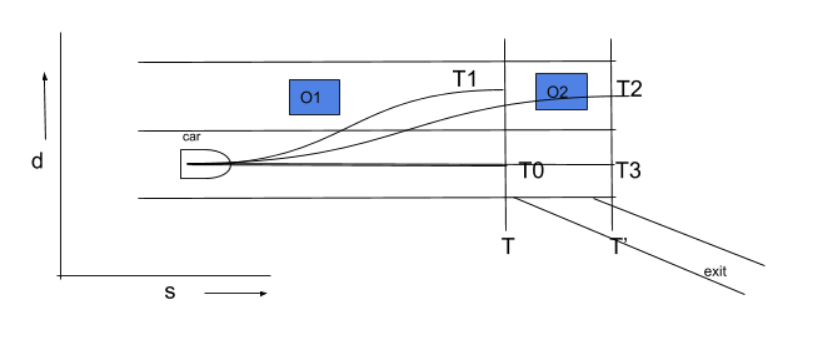
\includegraphics[width=0.8\textwidth]{Images/horizaon_optimality_2.png}
    \caption{Horizon Optimality reference}
    \label{horizon_optimality}
\end{figure}
 
 \todo{move to future works}
 Another horizon generally in discussion for a planner is spatial horizon which discusses how long is the path generated, as per this planning criteria at low velocities the spatial horizon considered is very small thus the planner may not make right decisions because of conditions like missing the obstacles ahead etc. This shortcoming can be improved by creating a spatial path with longer horizon in behavioral layer at lower speeds and allowing the local planner to follow new spatial path than following the global reference path. This is an efficient method as the path planning is generally less expensive than trajectory planning. As shown in figure \ref{optimized_reference}, following the original reference path(solid line) will lead to trajectories that turn a lot causing discomfort due to obstacles on the side of road that enter the road, thus by using an optimized reference path(dotted line), ego vehicle can plan efficiently even using short horizons.
 
 The resolution of the sampling in acceleration selection and lateral distance selection will also affect the optimality of planning, a chosen plan can only be optimal of the trajectories created by sampling, higher the number of samples, larger are the possibilities and a best selection is possible. 
 
 From the above discussion it can be stated that a planner that has a longer spatial horizon for path planning and short time horizons for trajectory planning will lead to an efficient planner. 
 
 \begin{figure}[h]
    \centering
    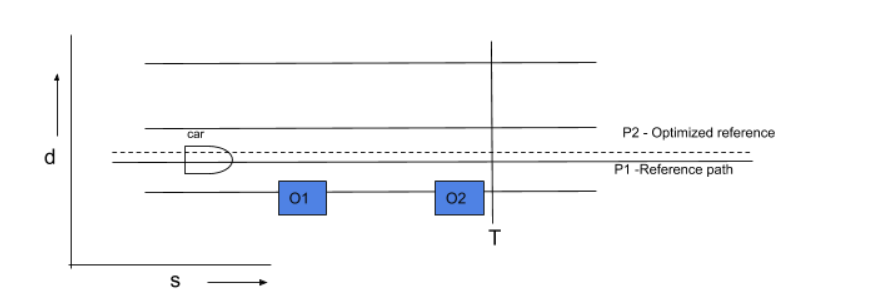
\includegraphics[width=0.8\textwidth]{Images/optimized_reference.png}
    \caption{Optimized Reference Path}
    \label{optimized_reference}
\end{figure}

\subsection{Feasibility}
\label{feasibility}
Ability of the vehicle to traverse the created trajectory determines feasibility, generally curvature of the path, smoothness and accelerations determine whether a trajectory is feasible or not. The proposed planner creates feasible trajectories at lower speeds because of the third order splines used, higher speeds require fifth or higher order splines to maintain continuity in path and speed. Discussions in \cite{cmu_parallel_thesis} \cite{ppt_teqniqs_coll_Avdnce} throw light on how to achieve higher degrees of smoothness, which approach is better in which driving conditions. As the intended application for this thesis is a modelcar, constant acceleration profiles are used due to limitation in ability of the car to track small changes in velocity and inaccuracies in measurement. These can be easily replaced by a smoother higher order polynomials with a better hardware platform. Consistency in paths evaluated with respect to previous plan is another factor in feasibility, the current planner penalizes trajectories deviating from previous plan and also takes into account current orientation of the vehicle in choosing a path. Thus creating smoother transitions from one state to another by respecting current driving orientation. 

\subsection{Completeness}
\label{completeness}
An algorithm is said to be complete if it can result in a solution every time. A motion planner can be called complete if it returns path if it exists in the space searched. Like many other sampling based approaches the planner proposed in this thesis only probabilistically complete. That is, probability of finding a solution approaches to one as the number of samples increases. If there are higher number of samples in the configuration space then higher are the chances of finding a solution. If a planner cannot find a solution within sampled region it forces the car to go into emergency manoeuvre. 

In Figure \ref{probablistically_complete}, there are only two sampled end states and there is no solution found by the vehicle, by increasing the number of lateral samples a solution can be easily found. In general condition of completeness can be improved in two ways, first is to sample as many points as possible and as closely as possible in the solution space. Second method is to keep on sampling till an end solution is found or timeout has been reached. The former method will reduce the computational performance while the later can be complex and expensive also. The planner proposed in this thesis implements a combination of both methods, as many samples as possible but evaluates only till a feasible solution is found. It is recommended to achieve completeness for safety purposes in autonomous driving. 

 \begin{figure}[h]
    \centering
    \includegraphics[width=0.8\textwidth]{Images/probablistically_complete.png}
    \caption{Probablistic Completeness}
    \label{probablistically_complete}
\end{figure}

\subsection{Runtime}

Though computation power is available cheaply, it is important to create solutions which are cheaper and can be employed in large scale. In this case sampling based approaches generally fare well and run on a low computational hardware. In contrast lattice based approaches such as \cite{cmu_parallel_thesis} \cite{diss_shui_phd_thesis} \cite{werling_frenet} computationally expensive and require a GPU to run. Low computational costs mean larger chances to be adopted to a greater number of platforms.

To compute the complexity of planner, lets consider $n_a$ denote the number of acceleration/deceleration profiles, $n_s$ denote the stopping deceleration profiles and $n_l$ denote the number of lateral distance samples. Then the maximum number of samples created is $(n_a+n_s)*n_l$, generally stopping profiles are less as at higher deceleration lower number of lateral samples are chosen due to limitations in vehicle dynamics. This thesis employs a hybrid combination of two methods mentioned in \ref{completeness} to achieve completeness. Therefore in best case only one trajectory is evaluated and complexity is $O(1)$ and the worst case complexity is $O((n_a+n_s)*n_l)$.

Trajectory evaluation with respect to dynamic obstacles is an expensive process in evaluation of trajectories, generally simulation based methods as discussed in  \cite{kolski_thesis} are generally expensive generally in terms of $O(n_o*n_n)$ where $n_o$ is the number of obstacles and $n_n$ is the number of simulation steps. This thesis employs a simple collision checking algorithm with constant time for evaluating one obstacle thus reducing the complexity to $O(n_o)$, number of obstacles. This process is not effective in intersections, currently a conservative approach to wait for other obstacles to pass is used, a simple approach as discussed in \cite{rrt_star} which has a performance better than the simulation based algorithms can also be employed in future.  

\todo{Write about the execution time for different number of samples, maximum execution time, minimum time from evaluation result etc}

\subsection{Deliberative Approach}
The planner proposed in this thesis maintains a mix of deliberative and reactive approach. Deliberative by evaluating a trajectory completely  before committing to it, this is important to create trajectories adhering to traffic, safe and comfortable. In general all the planners evaluate all the sampled trajectories then choose the best based on different costs. The planner proposed in this thesis does not follow this convention and once it finds a best trajectory it stops evaluating the other trajectories as presented in subsection \ref{traj_Selection}. This does not limit the real-time response of the trajectory as the sampling is chosen such that the worst case response time is within the hard real-time response required by the planner. 

%\subsection{Low Computational Costs}

%Though computation power is available cheaply, it is important to create solutions which are cheaper and can be employed in large scale. In this case sampling based approaches generally fare well and run on a low computational hardware. In contrast lattice based approaches such as \cite{cmu_parallel_thesis} \cite{diss_shui_phd_thesis} \cite{werling_frenet} computationally expensive and require a GPU to run. Low computational costs can enable the technology to be adopted to a larger market. Safety should not be compromised for sake of low computational costs and the planner proposed here employs large range of acceleration profiles to bring the vehicle to halt easily in case of an emergency.

%It is true that computation is cheaper in current generation but it is important to bring down the costs to bring technology closer to larger markets. All the lattice based planners which provide the best of the performance evaluate on an average of 100,000 trajectories in one planning cycle and depend on GPUs and many multicore processing units to achieve this results. On the other hand sampling based approaches are cheaper and more conservative. The planner proposed in \cite{cmu_parallel_thesis} can perform a double lane change evasive manoeuvre equivalent to professional drivers to avoid sudden obstacles.  



%\section{Comparisons to other Planners}

\todo{Comparison here doesn't make sense as there are no numbers to compare with other planners, theoretical comparisons can be presented in related work in forms of short comings in different planners. Here may be just add a table like in CMU or DISS shui thesis with comparision to other planner}

%All the motion planners proposed achieve similar objective of navigating smoothly on road with different special capability, these special techniques define how and where these planners can be used. It is tough to compare the planners performance by comparing in definite scenarios due to logistical constraints and costs and objectives of different planners. The generic parameters which define the performance of a trajectory planner are deliberative evaluation, higher dimensional search space, on-road, parallel, real-time. Different types of planners proposed achieve different goals and are suitable at different conditions. 

%\subsection{Comparison to Sampling based Approaches}
%There have been many sampling based approaches that are proposed as discussed in Section \ref{related_work} for trajectory planning. One of such approach is discussed in \cite{traj_smoothing}, here the authors differentiate between the path planning and velocity planning, this approach doesn't choose a spatial or temporal horizon before thus, at high speeds it may fall short if the sampled position is shorter and at low speeds the planned path is very far into the future such that the plan is not valid anyway after some time. This un-necessarily increases the complexity. 

%\subsection{Comparison to Lattice based approaches}
%As discussed in Section \ref{related_work}, lattice based approaches are expensive computationally(generally in terms of fourth order or more based on number of dimensions in lattice), they employ lesser number of acceleration profiles as discussed in \cite{cmu_parallel_thesis} \cite{diss_shui_phd_thesis} to reduce the complexity, this could be a real problem in driving in traffic scenarios where vehicles are close to each other with not so much space for evasive manoeuvres and hard breaking is needed. Though the planner proposed in this thesis cannot create single trajectory with multiple lateral shifts to perform evasive manoeuvres like any other sampling based approach proposed, this planner employs large number of accelerations and deceleration's to improve safety. These planners are designed to run on a separate hardware such as GPU and are not suitable for low computational platforms such as modelcar. 



%Advantages of combining path and velocity? - How it can reduce sampling state. 

%Acceleration profiles for emergency stopping 

%Simulation based approaches to the proposed approach in this planner for collision checking. 

%Why it is not important to validate other trajectories once the best trajectory is found. 

%Urban driving needs strong abilities to stop immediately and lattice planners cannot do this as the number of acceleration profiles increases the evaluated trajectories gets increased in thousands. 

%Eg: CMU - increasing one acceleration will add 13000+ more trajectories, discretizing time by one more step will add 200,000 thousand more trajectories to evaluate thus limit the spatial and temporal horizon the planner can evaluate. At high speeds a larger spatial horizon is needed but generally temporal horizon remains same at all the speeds thus we chose to plan in a temporal horizon to allow planning at all multiple speeds. 


%Divide the trajectory planning and behaviour layer, with this the complexity of solving the task can be reduced drastically. If the trajectory planner need not worry about the behaviours and focus solely on driving safely it will enhance the performance of the vehicle and achieve the costs at a low computational cost.  




\chapter{Conclusions and Future Work}
\label{conclusion}
\section{Conclusions}

\section{Future Work}
Replace by smoother polynomials over splines, especially in curves and when not following centre lane, they tend to be very bad. 

// Diss shui thesis - read though page 80 and understand further on benefits and demerits of polynomials vs splines. Add some in evaluation and some in future work


Prediction of state from where the planner should start planning instead of current position. 
Due to inaccuracies in current planners measurement of speed and acceleration it is tough to estimate where the vehicle will be when the planner is under execution. Currently based on assumption that the vehicle will follow the current path for next few ms, it is made offset in control node. This can be improved to have better synchronizaton between planner and controller. 


Create two functions to map lateral shift as a function of time and distance based on speed over current function only mapping based on distance.  

Use quintic polynomials at high speeds and cubic at low speeds. 


%\appendix

%\include{Chapters/Appendix1}

\bibliographystyle{plain}
\bibliography{Thesis}
%\usepackage{number}
%\bibliographystyle{acm}
%\bibliography{Thesis}

%\printnomenclature

%\cleardoublepage
%\begin{vcenterpage}
%\noindent\rule[2pt]{\textwidth}{0.5pt}
%\begin{center}
%{\large\textbf{My fancy title\\}}
%\end{center}
%{\large\textbf{Abstract:}}
%English version of the German ``Zusammenfassung''.\\
%
%{\large\textbf{Keywords:}}
%3-6 English keywords
%\\
%\noindent\rule[2pt]{\textwidth}{0.5pt}
%\end{vcenterpage}
%
%\clearpage
%\begin{vcenterpage}
%\noindent\rule[2pt]{\textwidth}{0.5pt}
%\begin{center}
%{\large\textbf{Mein schicker Titel\\}}
%\end{center}
%{\large\textbf{Zusammenfassung:}}
%Deutsche Version des Englischen ``Abstracts''.\\
%
%{\large\textbf{Keywords:}}
%3-6 deutsche Schl\"usselw\"orter
%\\
%\noindent\rule[2pt]{\textwidth}{0.5pt}
%\end{vcenterpage}

\end{document}
